%\documentclass[a4paper, english,10pt]{article}
%\documentclass[english,10pt, oneside, draft, a4paper]{report}
\documentclass[english,10pt, oneside, a4paper]{scrreprt}
%\usepackage[b5paper, layout=b5paper, textwidth=12cm, twoside,bindingoffset=1cm,outer=2cm,inner=2cm,includefoot,bmargin=3cm]{geometry}
\usepackage[a4paper, layout=a4paper, textwidth=12cm, bindingoffset=1cm,outer=2cm,inner=2cm,includefoot,bmargin=3cm]{geometry}
\usepackage[english]{babel}
\usepackage[utf8]{inputenc}
\usepackage[T1]{fontenc}
\usepackage{float}
\usepackage{subfig}
\usepackage{multirow}
\usepackage{tabularx}
\usepackage{perpage} % For å få fotnotenummerering til å starte på nytt for hver side
\usepackage{graphicx}
\graphicspath{{grafikk/}}
\usepackage[export]{adjustbox} %In including a figure, add "center" as a flag

\usepackage{epstopdf}
\usepackage{varioref}
\usepackage{listings} % For å vise frem kode på en bra måte
\usepackage{textgreek}
%\usepackage{tikz,pgfplots} % For å plotte Matlab figurer på en god måte
\usepackage{amsmath} % For å tilpasse ligninger til å vises over flere linjer
\usepackage{pdfpages} % For å legge til pdf i appendix delen
\usepackage{rotating}
\usepackage{hyperref} % [pdfborder=0]{hyperref} to remove borders around
% pdf-links.
%\usepackage[text={6.2in,9.5in},centering]{geometry}
\usepackage{mathtools}
\usepackage{color} % Farger i dokumentet

\usepackage{dialogue}

\linespread{1.5}

% \lstset{frame=shadowbox, rulesepcolor=\color{black}}
\lstset{numbers=left, frame=single, tabsize=2, breaklines=true}

\DeclarePairedDelimiter\abs{\lvert}{\rvert}%
\DeclarePairedDelimiter\norm{\lVert}{\rVert}%

\makeatletter
\let\oldabs\abs
\def\abs{\@ifstar{\oldabs}{\oldabs*}}
%
\let\oldnorm\norm
\def\norm{\@ifstar{\oldnorm}{\oldnorm*}}
\makeatother


\DeclareMathSymbol{\comma}{\mathpunct}{letters}{"3B} % Legger inn kommandoen \comma som komma i math mode

\hypersetup{%
    pdfborder = {0 0 0}
}

%\usepackage{endnotes}
%\usepackage[portrait, pdftex]{geometry}

\newcommand{\HRule}{\rule{\linewidth}{0.5mm}}
\pretolerance = 1414
\tolerance = 1414

\MakePerPage{footnote} % For å få fotnotenummerering til å starte på nytt for hver side
\labelformat{equation}{equation~(#1)}
\labelformat{figure}{figure~{#1}}
\labelformat{table}{table~{#1}}


% ########################################## 
%			Beginning of document
% ########################################## 

\begin{document}

% \title{Designing a software architecture for a motorsport driver information system}
% \author{Magnus Bae and Magnus Krane\\ NTNU}
% \date{December 2013}
% \maketitle
%\title{Piloting map service for navigating in punctuality analysis for trains \\ \vspace{2 mm} {\large A case study of railway
%operations}}\date{ June 17, 2014}


%\begin{titlepage}
%\begin{center}

%\vspace{10mm}
%
\includegraphics[width=0.55\textwidth]{logo_ntnu_eng.png}~\\[1cm]
% \vspace{30mm}

%\makeatletter
%    \parindent \z@
%    \reset@font
%    \vskip 40\p@
%    \par
%    \hrule height 2pt
%    \par
%    \vskip 4\p@
%    \huge \@title
%    \vskip 6\p@
%    \par
%    \hrule height 2pt
%    \par
%    \begin{flushright}
%      \large \@date \par
%    \end{flushright}
%    \vskip 100\p@
% \vspace{20mm}
%\begin{minipage}{0.4\textwidth}
%\begin{flushleft} \large
%\centerline{Magnus Krane}
%~\\
%\centerline{Supervisor:}
%\centerline{Sobah Petersen}
%\centerline{Co-supervisor:}
%\centerline{Andreas Dypvik Landmark - SINTEF}
%\end{flushleft}
%\end{minipage}
%\vfill
%\end{center}
%\end{titlepage}

\section*{Problem Description} % (fold)
\label{sec:_problem_description}

% section _problem_description (end)

\subsection*{Piloting map service for navigating in punctuality analysis for 
trains}

Conceptualize and develop prototype of map based visualizations of real time signal data to improve punctuality.



\setcounter{tocdepth}{5}
\setcounter{secnumdepth}{5}

%\includepdf[pages={-}]{signert_masterbeskrivelse.pdf} Eksempel på hvordan du legger inn pdf

\setcounter{page}{0}
\pagenumbering{roman}
% \pagedial{empty}

%Does the report contain the necessary elements as 
%abstract/summary, 
%table of 
%contents, 
%introduction, etc. in an appropriate form 

%starting point/objectives, 
%what is done and the 
%conclusions/results, and to maintain this overview throughout the reading. 

% #### Other stuff from the template

%%\title{Piloting map service for navigating in punctuality analysis for trains \\ \vspace{2 mm} {\large A case study of railway
%operations}}\date{ June 17, 2014}


%\begin{titlepage}
%\begin{center}

%\vspace{10mm}
%
\includegraphics[width=0.55\textwidth]{logo_ntnu_eng.png}~\\[1cm]
% \vspace{30mm}

%\makeatletter
%    \parindent \z@
%    \reset@font
%    \vskip 40\p@
%    \par
%    \hrule height 2pt
%    \par
%    \vskip 4\p@
%    \huge \@title
%    \vskip 6\p@
%    \par
%    \hrule height 2pt
%    \par
%    \begin{flushright}
%      \large \@date \par
%    \end{flushright}
%    \vskip 100\p@
% \vspace{20mm}
%\begin{minipage}{0.4\textwidth}
%\begin{flushleft} \large
%\centerline{Magnus Krane}
%~\\
%\centerline{Supervisor:}
%\centerline{Sobah Petersen}
%\centerline{Co-supervisor:}
%\centerline{Andreas Dypvik Landmark - SINTEF}
%\end{flushleft}
%\end{minipage}
%\vfill
%\end{center}
%\end{titlepage}

\section*{Problem Description} % (fold)
\label{sec:_problem_description}

% section _problem_description (end)

\subsection*{Piloting map service for navigating in punctuality analysis for 
trains}

Conceptualize and develop prototype of map based visualizations of real time signal data to improve punctuality.



%\addcontentsline{toc}{section}{Preface}
\section*{Preface}

The work of this thesis has been performed at the Department of Computer and
Information Science (IDI) at the Norwegian University of Science and Technology
(NTNU), and in collaboration with SINTEF Technology and Society during the
spring semester of 2014. \\

During the work of this thesis, I have been supervised by Sobah Abbas Pettersen
and co-supervised by researcher Andreas Landmark (SINTEF), research manager
Andreas Seim (SINTEF), and researcher Rimmert van der Kooij (SINTEF), who have
all been a great help throughout the process, providing valuable input and
guidance.

I would also like to thank fellow students Magnus Bae and Bjørn Thomas Vee for
feedback and help when needed.\\

I have also been part of the student organization Revolve NTNU this semester,
which is a group of students building a prototype formula student race car for
participating in the international Formula Student competitions. I would like
thank my fellow team members for participating in some of the best times I have
experienced.

A final thank you to my supervisors for understanding that participating in
Revolve NTNU has made time difficult to balance.

\mbox{}\\[1pc]
Trondheim, \today\\
\mbox{}\\[1pc]
Magnus Krane

\clearpage

%\addcontentsline{toc}{section}{Summary}
\section*{Summary}

		XXX

\clearpage

%\addcontentsline{toc}{section}{Norwegian Abstract}
\section*{Sammendrag (Norwegian Abstract)}

I et komplekst system som det norske jernbane nettverket er det mye som kan
påvirke punkligheten til et tog. Operatørene på jernbanen streber etter å oppnå
høyere og høyere punklighet. Infrastruktur eier, Jernbaneverket,  streber etter
minst mulig nedetid på trafikk nettverket.
Ved å analysere og sammenligne forskjellige data sett er det mulig å forstå grunnen til forsinkelsene.
%Setning for å henge sammen over og under kommentar
Ulike brukere har forskjellig behov når de studerer data settene. For eksempel
så har en direktør behovet for å kunne se hele bildet, mens
strekningsansvarlige har behov for å kunne studere hver minste detalj.\\

I denne masteroppgaven skal demonstrerer vi et system som tar hensyn til de
forskjellige brukerene sine behov for forskjellig presentasjon av data.
Systemet tar også hensyn til behovene for å kunne se på forskjellige data
og sammenligne disse.
	
\clearpage


\renewcommand\listfigurename{List of Figures}
\listoffigures
\clearpage
% \renewcommand\listtablename{List of Tables}
% \listoftables
\clearpage
\renewcommand\contentsname{Table of Contents}
\tableofcontents

\setcounter{page}{0}
\pagenumbering{arabic}

% !TEX root=../thesis.tex

\chapter{Introduction}

In this report we aim to design a software architecture for a driver information
system\footnote{Also known as In Vehicle Information System, IVIS}
that is to be prototyped and installed in a formula student race car. We will
also discuss the state of the art, technological alternatives and introduce
background information pertaining to the domain and use-cases.

To design this architecture we have undertaken a significant literature study
of both architectural design patterns and driver/operator information systems.
We have looked at what a typical driver information system does, how it does
it, and what the state of the art is. Other fields employing information 
systems to provide vehicle operators with real-time information have also been
studied.

This research effort is made to serve as a foundation to build a prototype
driver information system in collaboration with Revolve NTNU (Revolve), a 
student organization  created by students at the Norwegian University of 
Science and Technology.
The the collaboration with Revolve will serve as a testing ground for our 
design and allow us to test its feasibility in the
context of motorsport.

For the last three years Revolve has been hard at work building formula style race
cars to participate in events of the international motor sport competition series
``Formula Student'' (FS). The competitions are arranged by the Institution of Mechanical Engineers. In the competitions teams of students compete against each other
with small formula-style cars they have designed and built from scratch. There are
disciplines that involves racing the cars as well as disciplines in business,
design, and cost. The combined score from these events decide the official
results, but there are also prices awarded for excellence in different fields

Motorsport has for many years been a testbed for car manufacturers and a lot of
technology that we today take for granted has come to fruition through motorsport. However
ordinary cars have seen larger leaps in technology with regards to information
consumption than cars built for motor racing. For some years some high-end cars
have even been equipped with heads-up displays (HUD) that allows the driver to 
keep focus on the road instead of looking down at the instruments \cite{wiki:hud},
and it is becoming more and more common.

Despite great developments in automobile technology over the past 50 years little
has changed in the way that motorsport drivers receives information during an
event. There are displays, gauges, and other visual indicators\footnotemark[1]
, in addition to radio-communication \cite{wiki:formula_radio} if that is allowed in the competition. The technology under the hood
has become much more advanced, but the amount of information you can
convey to the driver still seems to be very limited; the pace is just too high
to be able to keep moving focus from the road (see appendix \vref{interview:bakkom}).

Driver information systems in the context of motorsport is a field neglected by
science (see \vref{background:rel_reasearch}). There has been done some
research around driver information systems in commercial vehicles and normal 
passenger cars, most of which involve studies of heads-up display technology or
use.

This is therefore a field where we are threading into new territory. 
Requirements are hard to elicit up front, and we don't know
from the start what is a good design for such a system. It is quite possible
that requirement changes can come from opportunities enabled by 
creating a new system that can potentially deliver more information to the
driver with faster response times (from the driver) and less distractions. 
This means that any system developed must be flexible enough to allow for easy 
experimenting with configuration
alternatives and have a high-level support for requirements evolution.

The question we want to address in this report is as follows; How can we
enable the development of a state of the art computerized driver information system
by creating a software architecture that is flexible enough to allow easy
experimenting and customization?

The rest of this document is divided into several parts. In the background chapter we will
discuss the collaboration with Revolve NTNU and present the Formula Student
competition. We also present relevant electronic principles and knowledge and discuss the current
state of research with a focus on automotive information systems. Chapter \vref{chapter:method}
introduces the methods we've applied in our work, while
the following chapter (\vref{chapter:results}) shows the findings of our research.
Then we discuss our findings and try to put them in perspective in chapter \vref{chapter:discussion}, before we move
onto the conclusion and discussing recommendations and possibilities for
further work in chapter \vref{chapter:conclusion}.
The appendices contain development artifacts created during the design process
and details the results and the information they build upon, as well as an interview with a driver from last years Revolve-team. 


\footnotetext{
	Although extensive research has been performed scientific, 
	findings are rare. Cottle et al.. \cite{wirelessDashboard} discusses implementing a 
	wireless ``dashboard'' (controls and instruments on a steering wheel). 
	Although lacking scientific base the statement should hold; this 
	assumption is made stronger by analyzing motorsport on TV and for 
	pictures of race cars' interiors.
}

%\chapter{Definitions \& abbreviations}
%%Abbreviations and definitions
\label{sec:abbriv}
\vspace{5mm}

\begin{description}
\item [GIS] Geographic information system
\item [Regularity]	Jernbaneverket defines regularity as the number of trains that gets run as planed in the time schedule. 
\item [Uptime]	Jernbaneverket states that uptime in regards to punctuality defines from hours of delay caused by infrastructure relative to sum of planed train hours per year. \begin{equation} Uptime =
\frac{\text{Train hours - hours of delay}}{\text{Train hours}}\times 100 \end{equation}
\end{description}



% !TEX root=../thesis.tex

\chapter{Background}
\label{chapter:background}

A train network is a complex system. Almost every running train have the 
possibility to affect almost every other train running in the system.  When 
you look at a busy area, such as a major city and it's closest
area, a great deal of trains can be on the move at any given time on a
railway network with limited capacity. This leads to limited time slots for each 
train and every problem can lead to major delays.


Even though one train may be experiencing delay, this delay may be part of a
sequence of problems that can be tracked back to a seemingly unrelated part of
the the network and a perhaps a bad decision there\cite{cule2011mining}. \\

In the Norwegian railroad a train is on schedule if it arrives the final
destination within a margin on 3 minutes and 59 seconds, if it is a long
distance train the margin is 5 minutes and 59 seconds. 
Jernbaneverket (see\vref{sub:subsection_jernbaneverket}) defines regularity as the number of trains that gets run as 
planed in the time schedule. 
Uptime in regards to punctuality is defined by Jernbaneverket from the hours of delay\footnote{Hours of delay due to infrastructure excluded traffic	management and external conditions} caused by infrastructure relative to sum of planed train hours\footnote{Planed train hours (passenger and freight trains)} per year.
\cite{jernbaneverketPunklighetsTall}
\begin{equation} Uptime =
		\frac
				{
					\text{Train hours - Hours of delay}
				}
				{
					\text{Train hours}
				}\times 100 
\end{equation}\\

As Landex\cite{landex2009gis} says, there exist few GIS-approaches concerning
visualization of railroad capacity. Both the visualizations shown by Landex and
in section \vref{sect:backgroundExamples} only seems to take into consideration if
the trains are delayed, and the amount of delay. 

However, to minimize the delays all over the railway network, it may be necessary
to not only see that certain routes are delayed but also why it is delayed. To
be able to understand this, you need to be able to mine data from the railway
network administrator and have a good visualization tool to present it. 

\pagebreak
\section{Examples}
\label{sect:backgroundExamples}

\subsection{Zugmonitor}
\label{sub:subsection_zugmonitor}

In the Zugmonitor (see \vref{fig:zugmonitor}) example each long-distance 
trains in the German railway network has been plotted as a arrow on a German 
map. To illustrate the punctuality of each train, a colored circle has been 
added to each arrow if the train is delayed with varying color depending on 
how big the delay is. It has also been implemented a time line functionality 
to see how the trains are on each step of the routes. This time line 
functionality has both a play forward function and manually drag along the 
time line.

\begin{figure}[!htbp]
	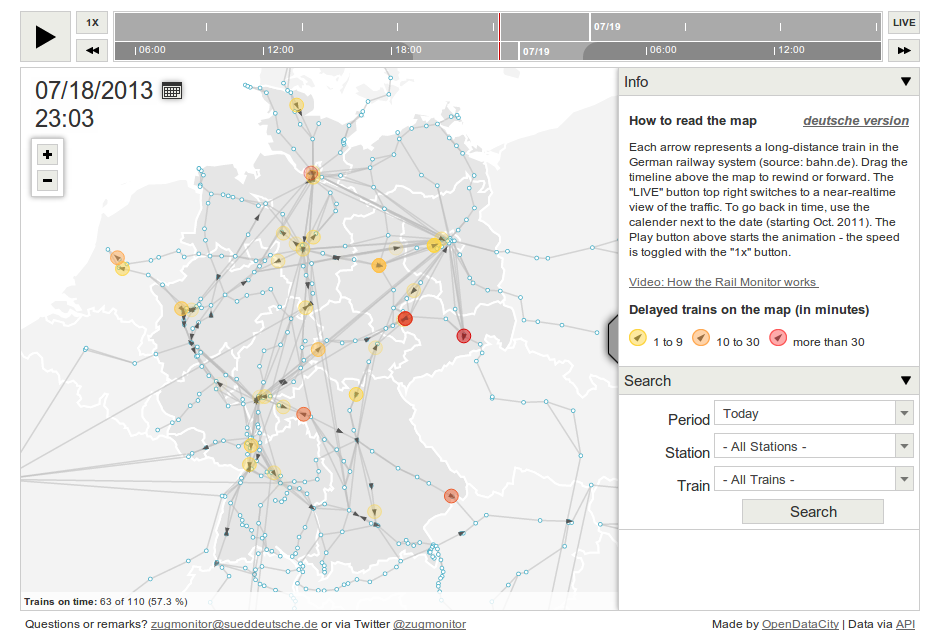
\includegraphics[width=\textwidth,center]{zugmonitor.png}
	\caption[Zugmonitor]{Zugmonitor \cite{zugmonitor}}
	\label{fig:zugmonitor}
\end{figure}
\pagebreak

\subsection{Vaguely live map of trains in the United Kingdom}
\label{sub:subsection_ukLiveMap}

This is a map which plots the relative location of each train in the United
Kingdom (see \vref{fig:ukLiveMap}). The plot fetches the departure time from the 
National Rail website and calculates the relative location. The plot does not
indicate whether or not the trains are on schedule or delayed, this must be
done either manually or for instance checking a time table\cite{trainTimesUK}.
Both the map and time table is developed on hobby basis by the same person. 

\begin{figure}[!htbp]
	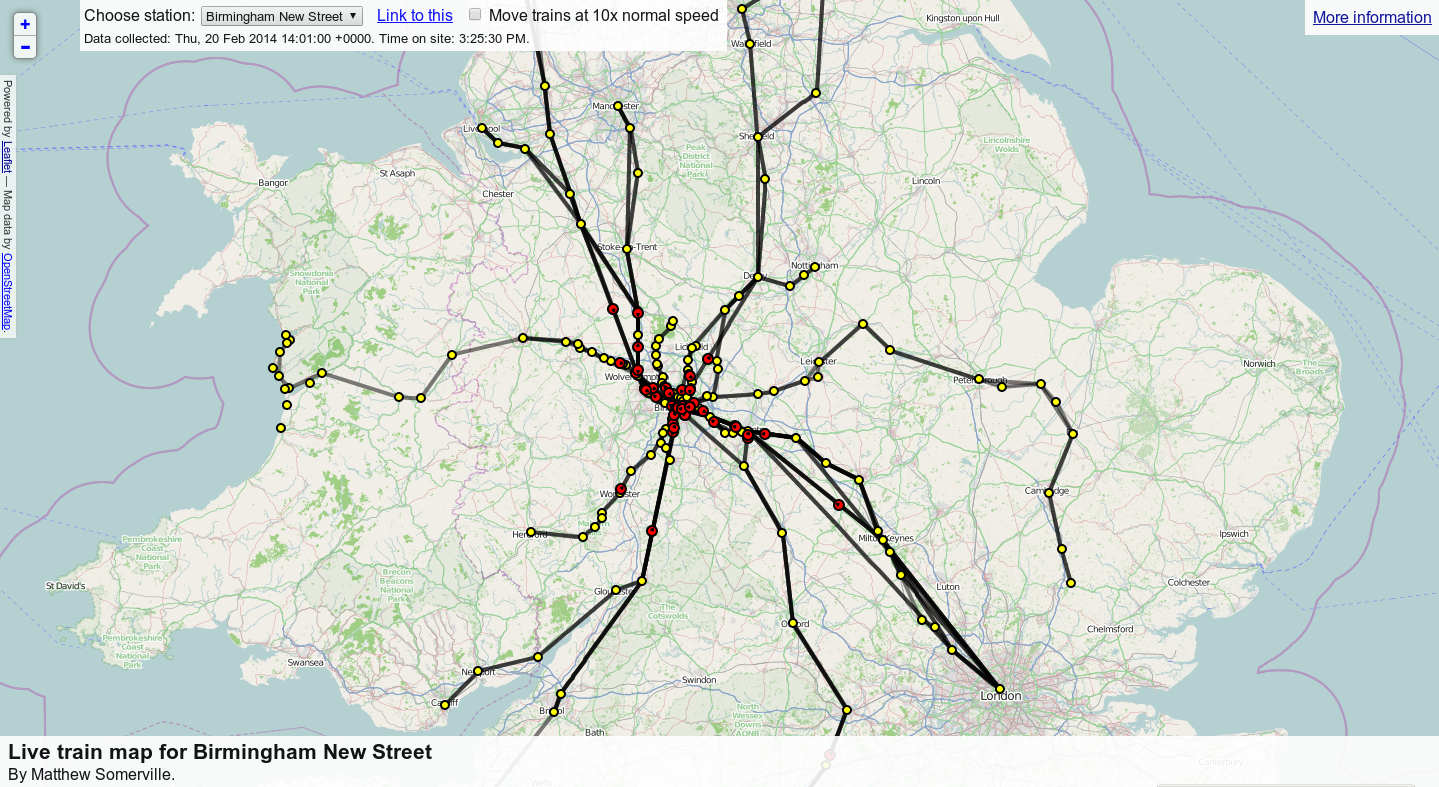
\includegraphics[width=\textwidth,center]{live-train-map-for-Birminingham-new-street.png}
	\caption[Vaguely live map of trains in the United Kingdom]{Vaguely live map of trains in the United Kingdom \cite{ukLiveMap}}
	\label{fig:ukLiveMap}
\end{figure}
\pagebreak

\subsection{MUNI Light Rail}
\label{sub:subsection_muniLightRail}

This a train graph based on the N-Judah line on the Muni Metro light railway line in San Francisco (see \vref{fig:muniLightRail}). 
This chart plots the schedule of the each train and the actual time each train 
uses. The chart auto updates each 10 seconds, and combined with being able 
to spot the difference between the schedule and the actual time, makes it easy 
spot the delay of each train. As with \vref{sub:subsection_ukLiveMap} it has been 
developed on a hobby basis.

\begin{figure}[!htbp]
	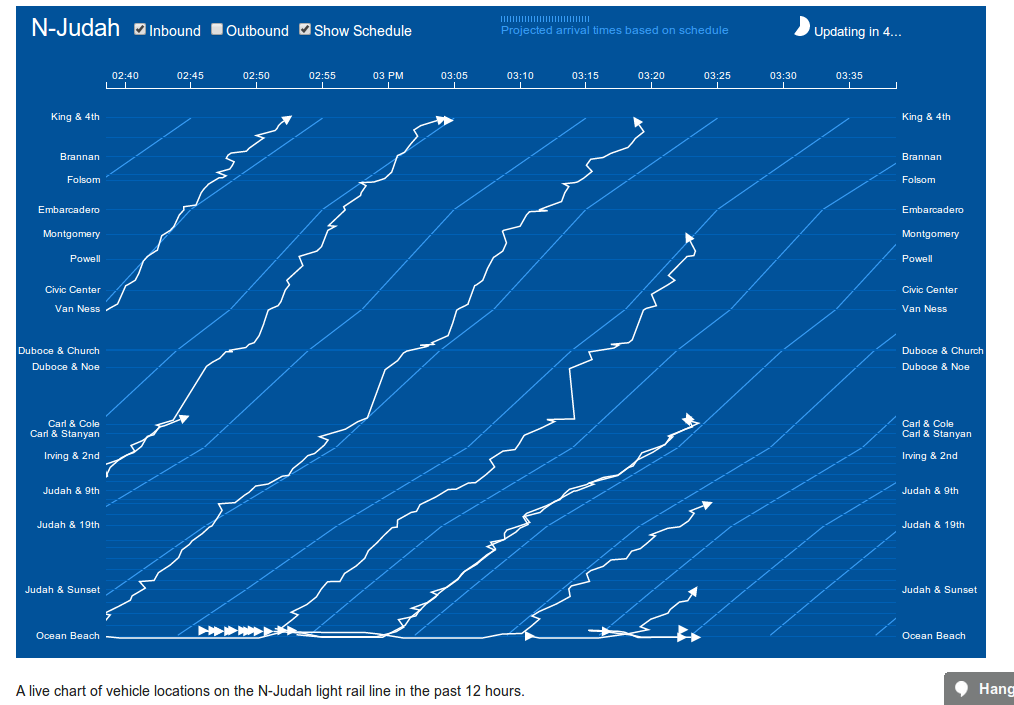
\includegraphics[width=\textwidth,center]{visualizing-transit-delays.png}
	\caption[Visualizing transit delays]{Visualizing transit delays \cite{muniLightRail}}
	\label{fig:muniLightRail}
\end{figure}
\pagebreak


\subsection{MiseryMap}
\label{sub:subsection_zugmonitor}

The MiseryMap (see \vref{fig:miserymap}) shows how much different airports and 
the routes between them are delayed. It also have a playback function to see
how the delays are throughout the day. This plot also shows some weather so it
may be possible to spot if the delays to be blamed on uncontrollable
conditions. 

\begin{figure}[!htbp]
	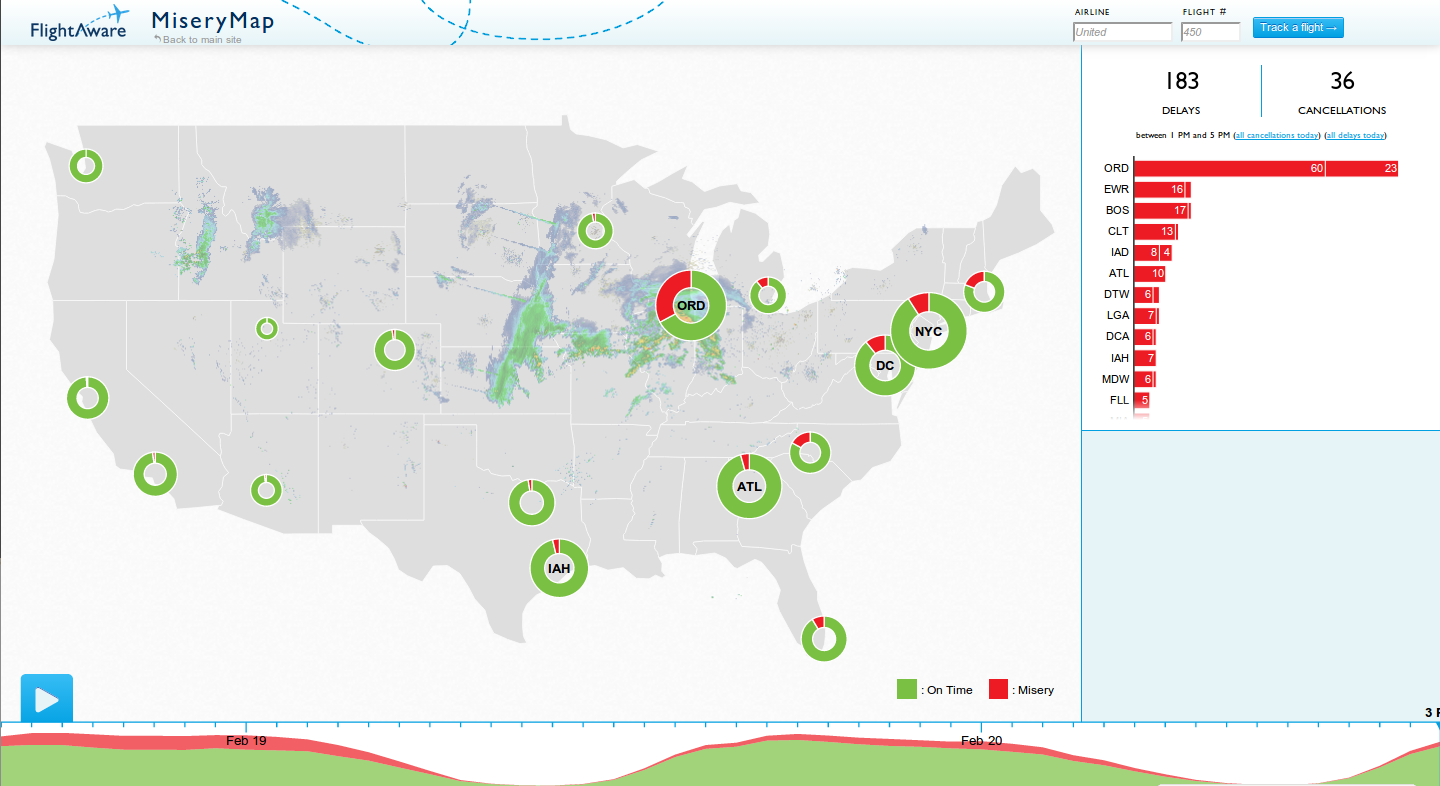
\includegraphics[width=\textwidth,center]{MiseryMap.png}
	\caption[MiseryMap]{MiseryMap \cite{flightAware:MiseryMap}}
	\label{fig:miserymap}
\end{figure}
%\pagebreak
 
\subsection{Jernbaneverket}
\label{sub:subsection_jernbaneverket}

Jernbaneverket is the Norwegian governments agency for railway services \cite{jernbaneverketAbout}.
This means that they are responsible for all the railway network in Norway.
Because of this, they also collect in data from points that each train passes. 
Based on this, they have recently released a map (see \vref{fig:jernbaneverket-punklighet}) over the punctuality on each stretch. This is a 
interactive map which shows a pop-up box containing the punctuality of the 
stretch clicked on, and this pop-up also shows which routes are using this 
stretch. The map, does not however, show more information if the user zooms 
inn, which is possible within the map itself, and has a static view of Norway 
and the railway. This map only shows the punctuality for passenger trains, and
not freight trains and/or both. 

To analyze each stretch, on a detail level of between each station,
Jernbaneverket has a internal system called TIOS (see \vref{fig:jernbaneverket-tios}).
This is a train graph which plots all trains that passes between all stations,
in this example between Oslo S and Drammen, where the red lines means delays
and the red circle indicates a reason code. XXX

\begin{figure}[!htbp]
	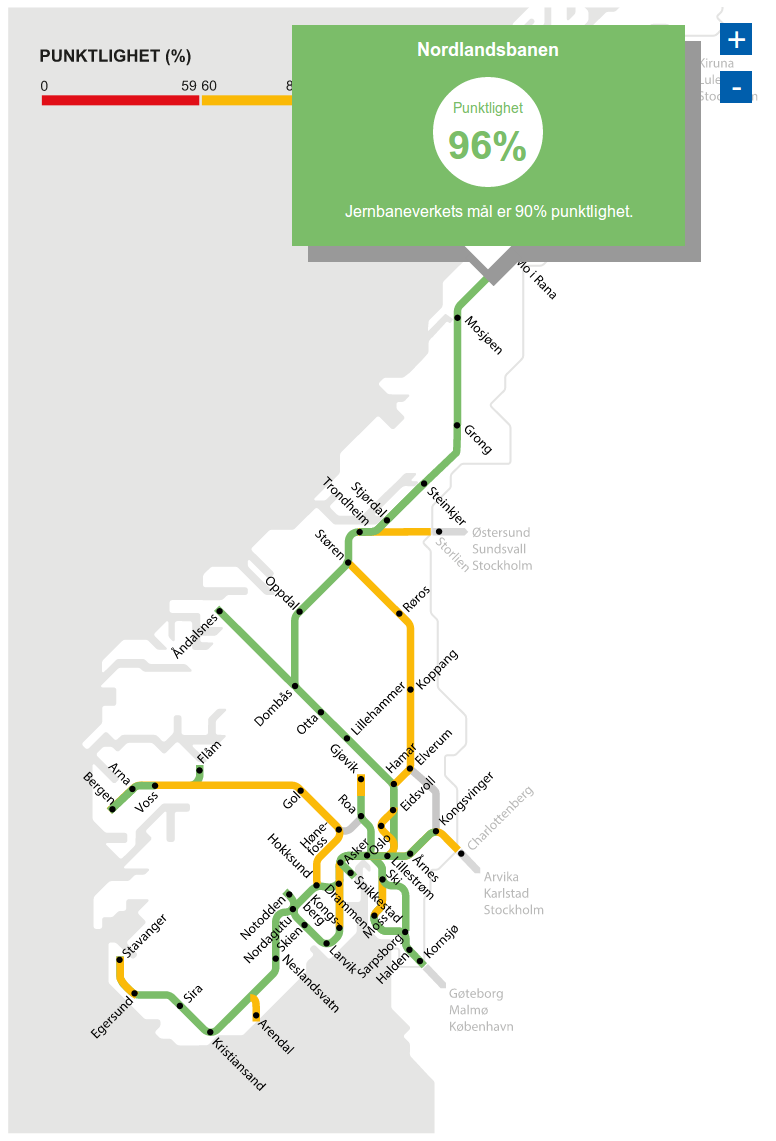
\includegraphics[height=\textheight,center]{jernbaneverket-punklighet.png}
	\caption[Punctuality map for Norwegian railway]{Punctuality map for Norwegian railway
	\cite{jernbaneverketPunklighetKart}}
	\label{fig:jernbaneverket-punklighet}
\end{figure}
\pagebreak

\begin{figure}[!htbp]
	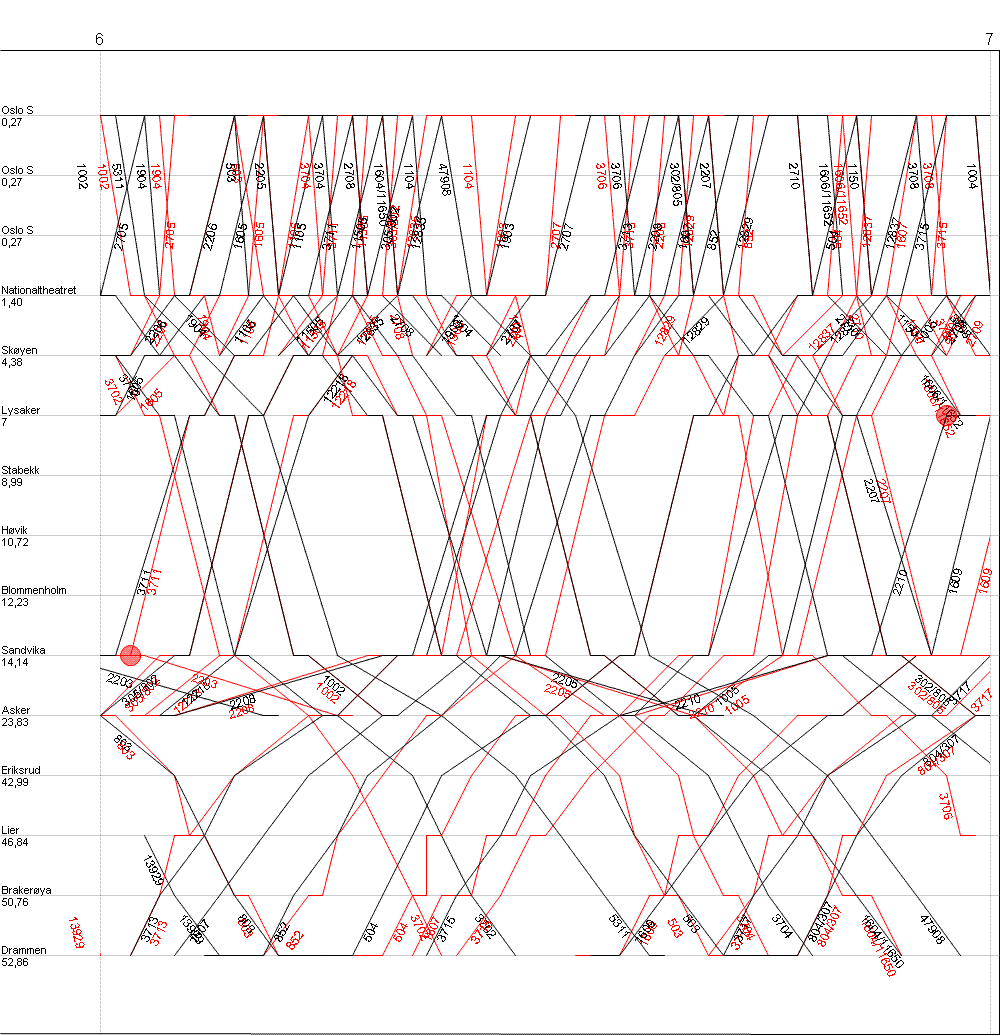
\includegraphics[width=\textwidth,center]{tios.png}
	\caption[TIOS]{TIOS\cite{jernbaneverketPunklighetKart}}
	\label{fig:jernbaneverket-tios}
\end{figure}
\pagebreak


\subsection{Tåg.info}
\label{sub:subsection_taag.info}

\begin{figure}[!htbp]
	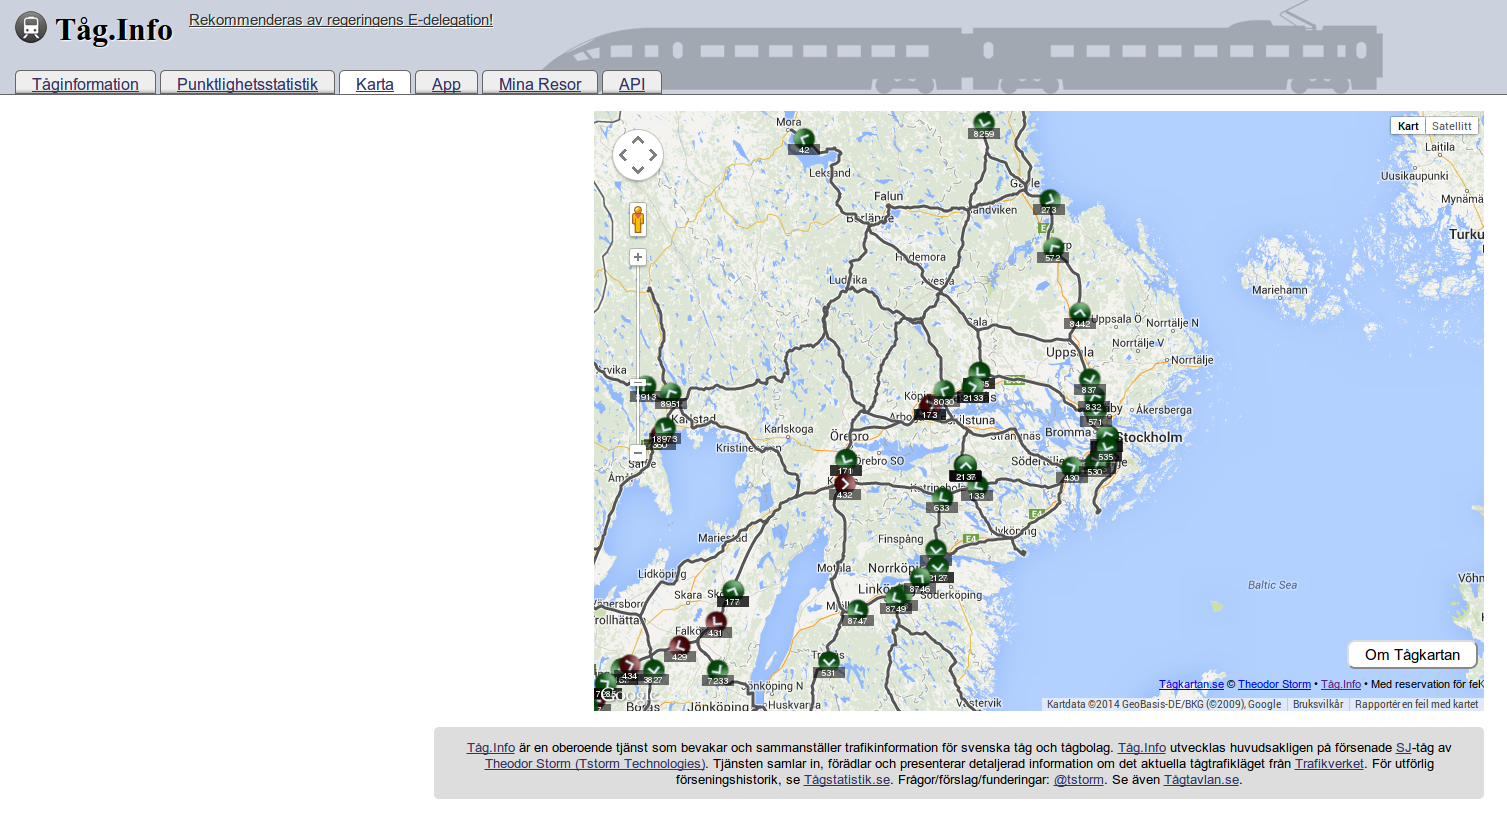
\includegraphics[width=\textwidth,center]{taag-info-kart.png}
	\caption[Tåg.info kart]{Tåg.info kart
	\cite{taagInfo}}
	\label{fig:taag-info-kart}
\end{figure}
\pagebreak

\begin{figure}[!htbp]
	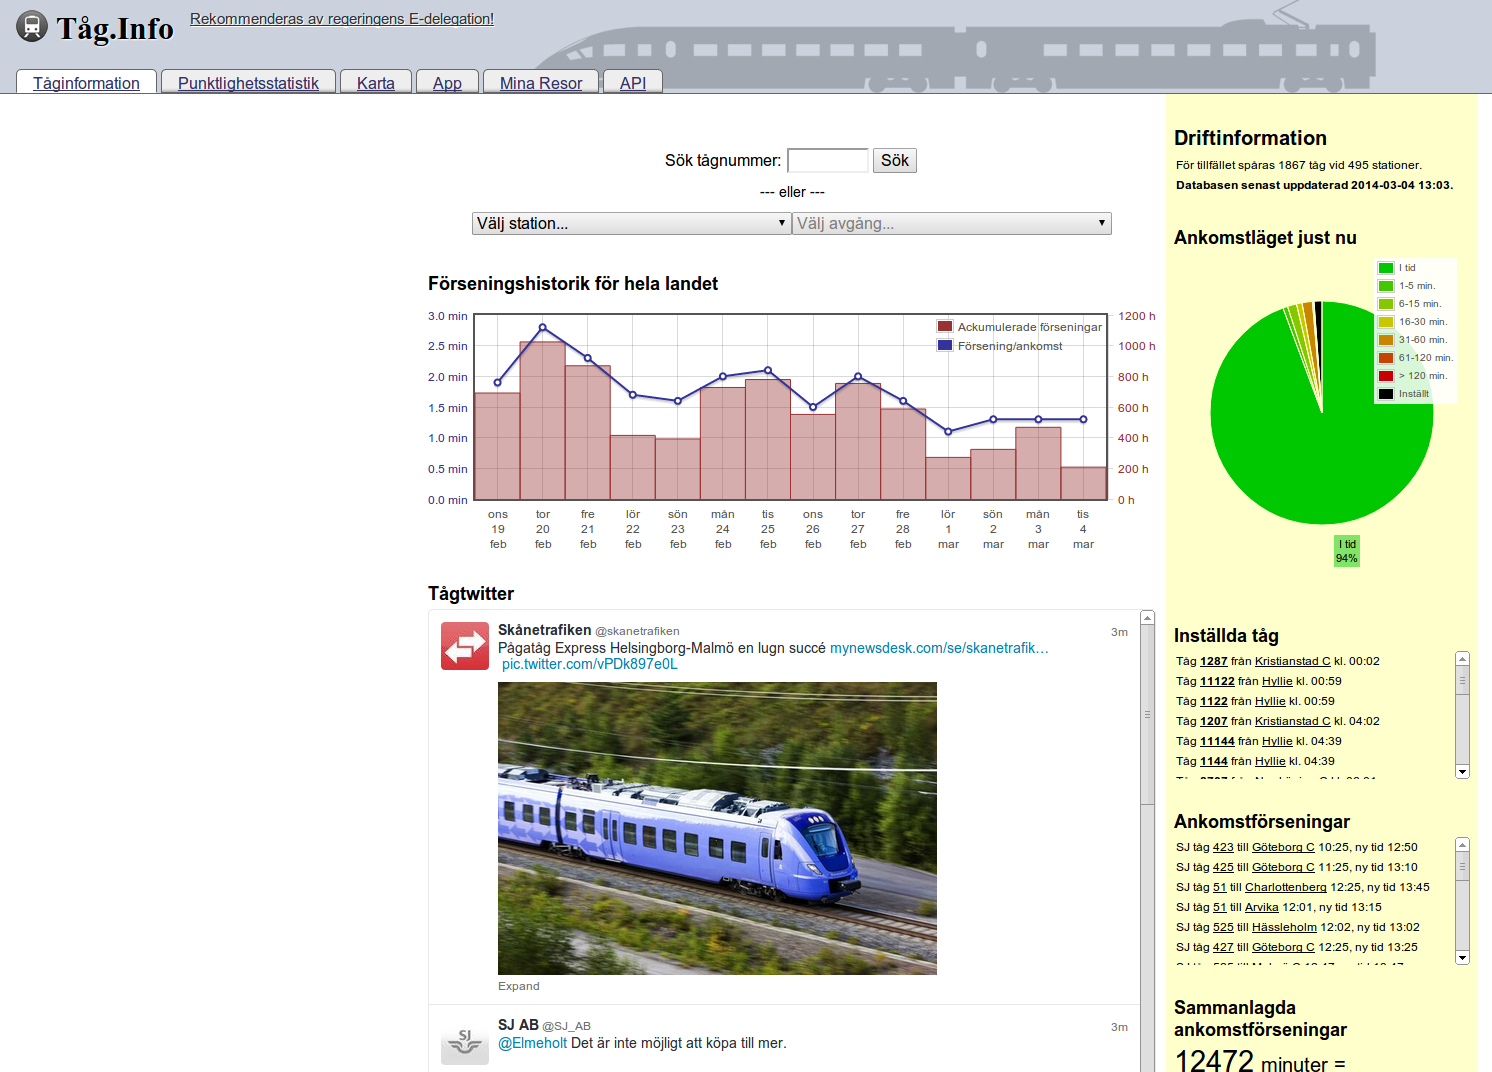
\includegraphics[width=\textwidth,center]{taag-info-historik.png}
	\caption[Tåg.info history]{Tåg.info history
	\cite{taagInfo}}
	\label{fig:taag-info-kart}
\end{figure}
\pagebreak


\subsection{SINTEF Presis}
\label{sub:subsection_sintefPresis}

The PRESIS\cite{sintefPresis} project is a project between SINTEF\cite{sintef},
Transportøkonomisk Institutt\cite{transportOkonomiskInstitutt},
NTNU\cite{ntnu}, Jernbaneverket(section \vref{sub:subsection_jernbaneverket}) and the train operators. It is meant to
systematicly improve the precision level in the railway system by developing
methods, tools, and processes. In this project it has been developed several
prototypes for analyzing train delays. 

If you look at \vref{fig:kjoretidstes-strekning}, it is possible to analyze the
difference in density between two selectable stations on two different,
selectable time periods. 

When looking at \vref{fig:krysningsinteraksjon}, it is possible to see how one
train might affect another at a selected station, plotted based on how much
both trains are delayed from -1 to 20 minutes. 



%\begin{figure}[!htbp]
%	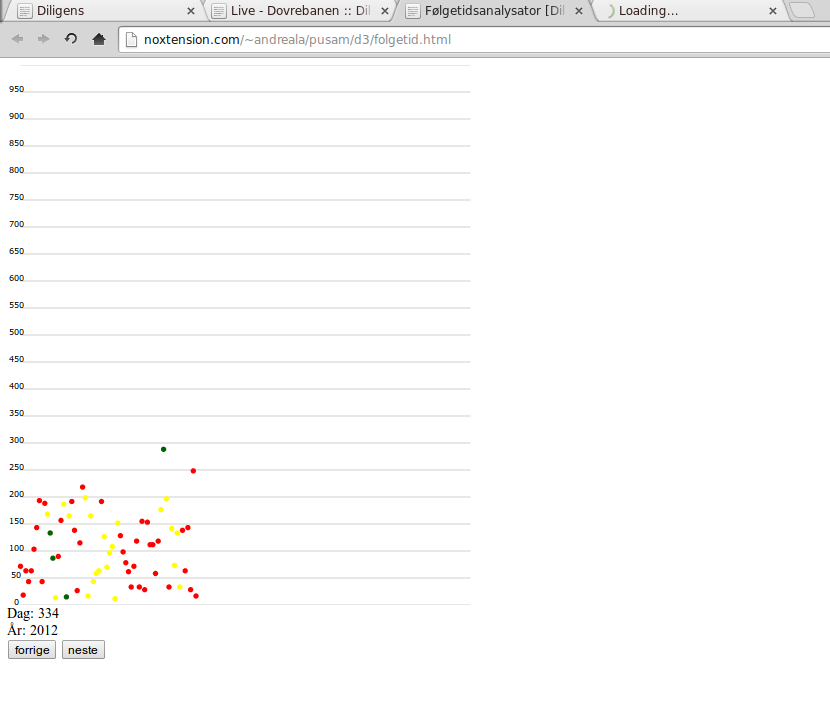
\includegraphics[width=\textwidth,center]{folgetid.png}
%	\caption[folgetid]{folgetid \cite{sintefPresis}}
%	\label{fig:folgetid}
%\end{figure}
%\pagebreak

\begin{figure}[!htbp]
	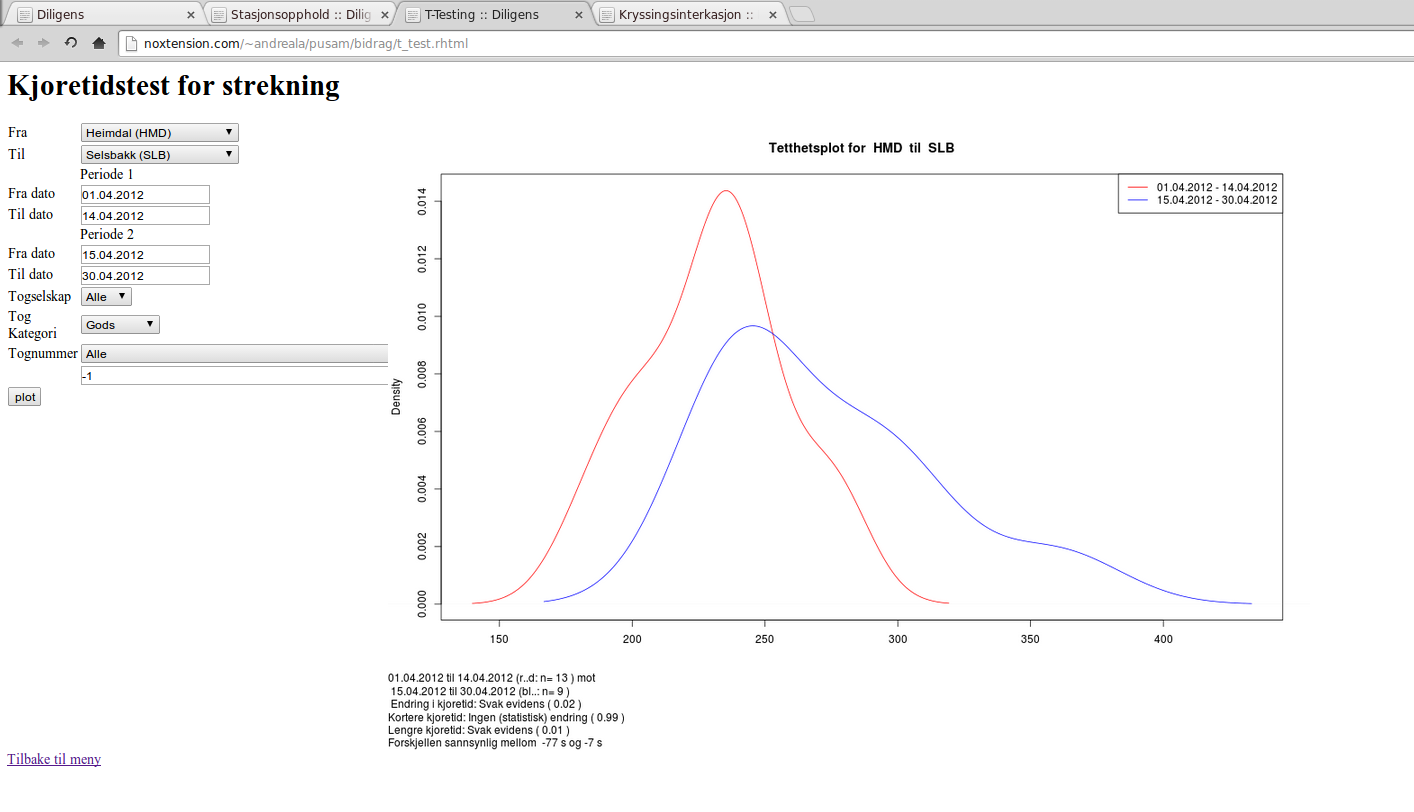
\includegraphics[width=\textwidth,center]{kjoretidstes-strekning.png}
	\caption[Density plot based on driving time]{Density plot based on driving time \cite{sintefPresis}}
	\label{fig:kjoretidstes-strekning}
\end{figure}
\pagebreak

\begin{figure}[!htbp]
	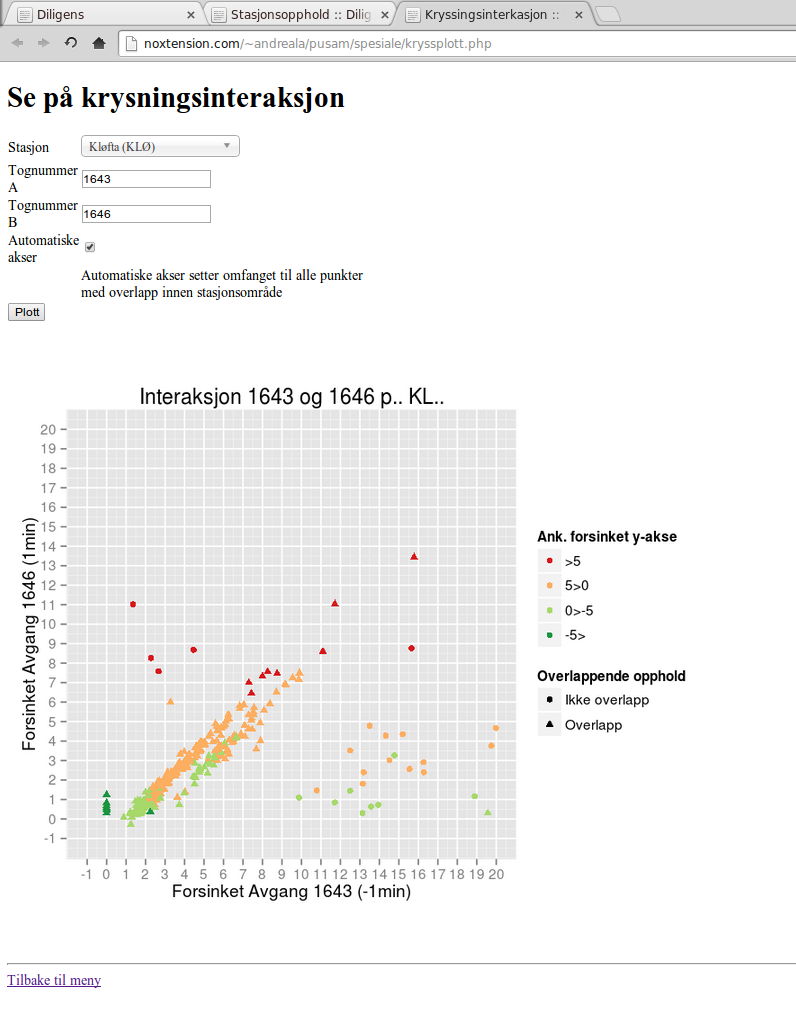
\includegraphics[width=\textwidth,center]{krysningsinteraksjon.png}
	\caption[Train interaction plot]{Train interaction plot \cite{sintefPresis}}
	\label{fig:krysningsinteraksjon}
\end{figure}
\pagebreak

\begin{figure}[!htbp]
	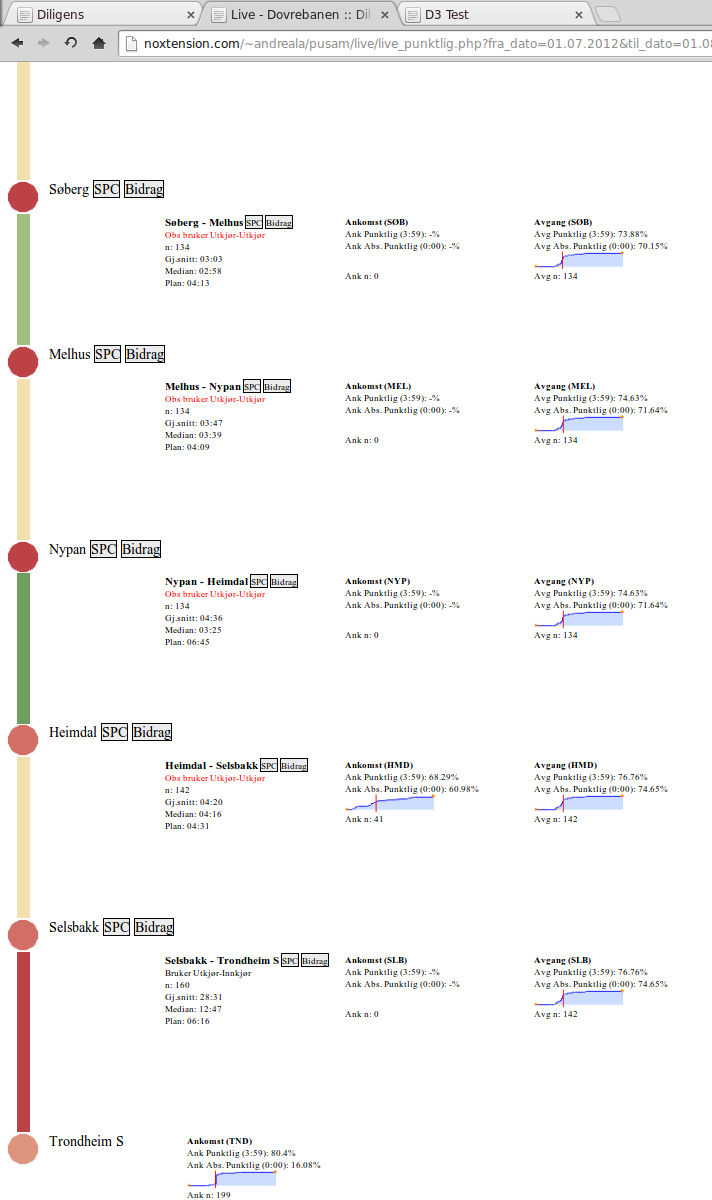
\includegraphics[height=\textheight,center]{live-punklighet.png}
	\caption[Punctuality for routes]{Punctuality for routes \cite{sintefPresis}}
	\label{fig:live-punklighet}
\end{figure}
\pagebreak

\begin{figure}[!htbp]
	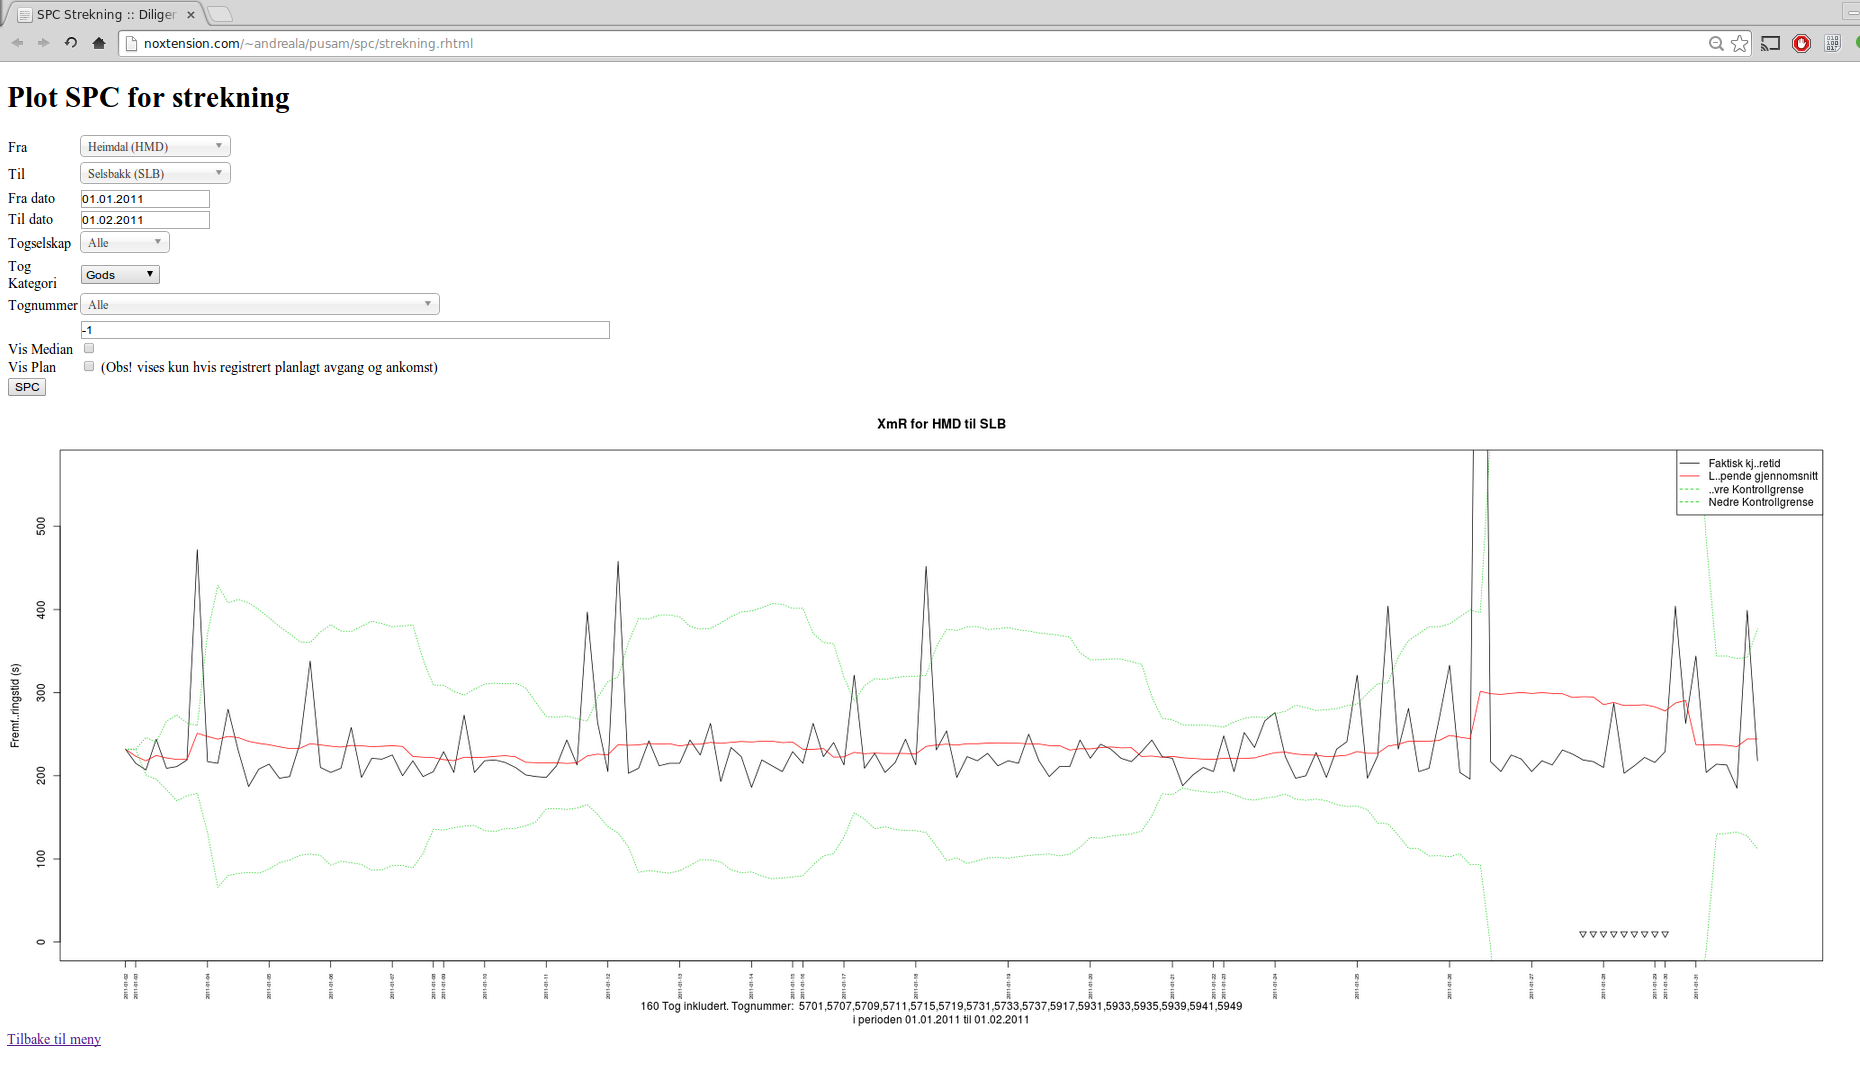
\includegraphics[width=\textwidth,center]{plot-spc-for-strekning.png}
	\caption[Time over distance plot (SPC)]{Time over distance plot (SPC) \cite{sintefPresis}}
	\label{fig:plot-spc-for-strekning}
\end{figure}
\pagebreak

\begin{figure}[!htbp]
	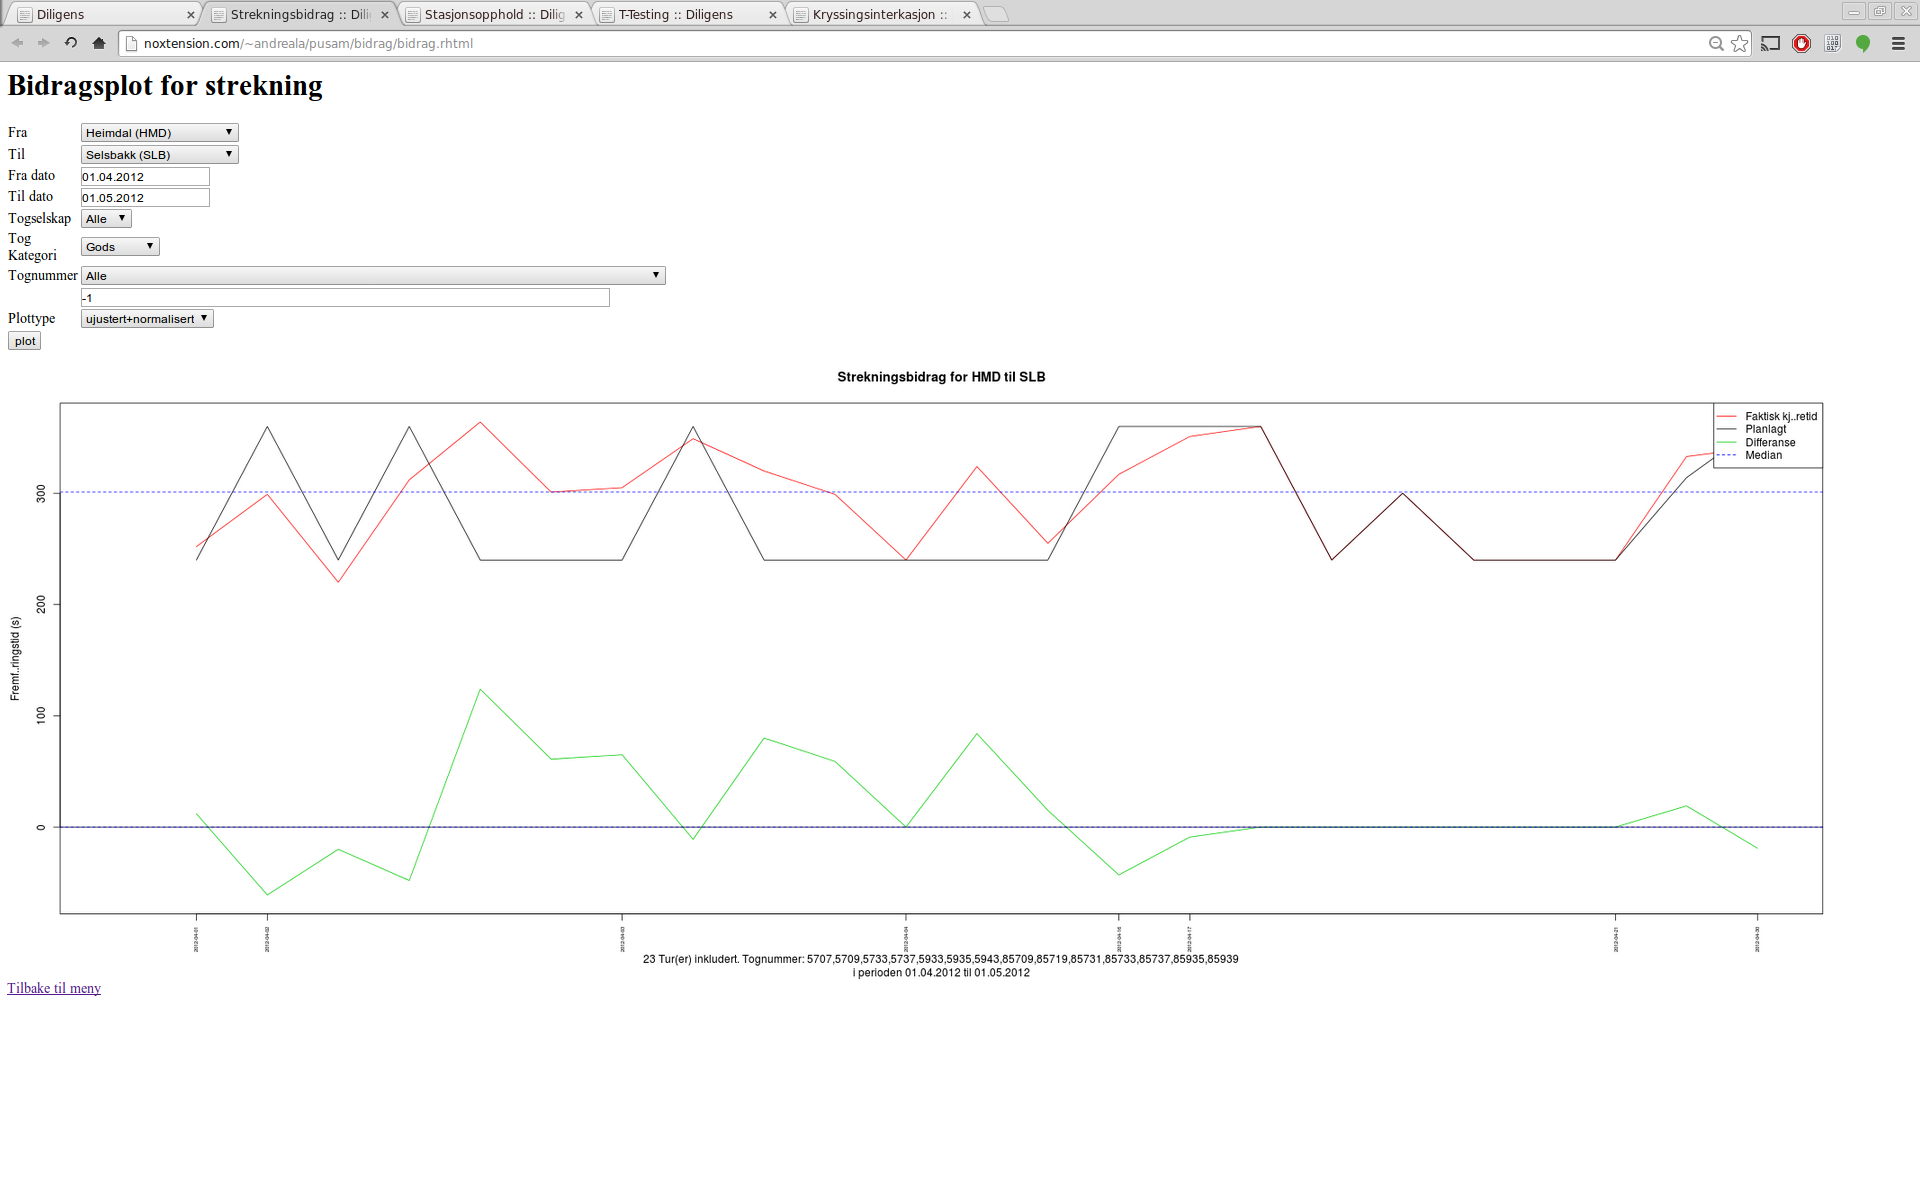
\includegraphics[width=\textwidth,center]{bidragsplot-strekning.png}
	\caption[Time over distance plot (Bidrag)]{Time over distance plot (Bidrag) \cite{sintefPresis}}
	\label{fig:bidragsplot-strekning}
\end{figure}
\pagebreak

\begin{figure}[!htbp]
	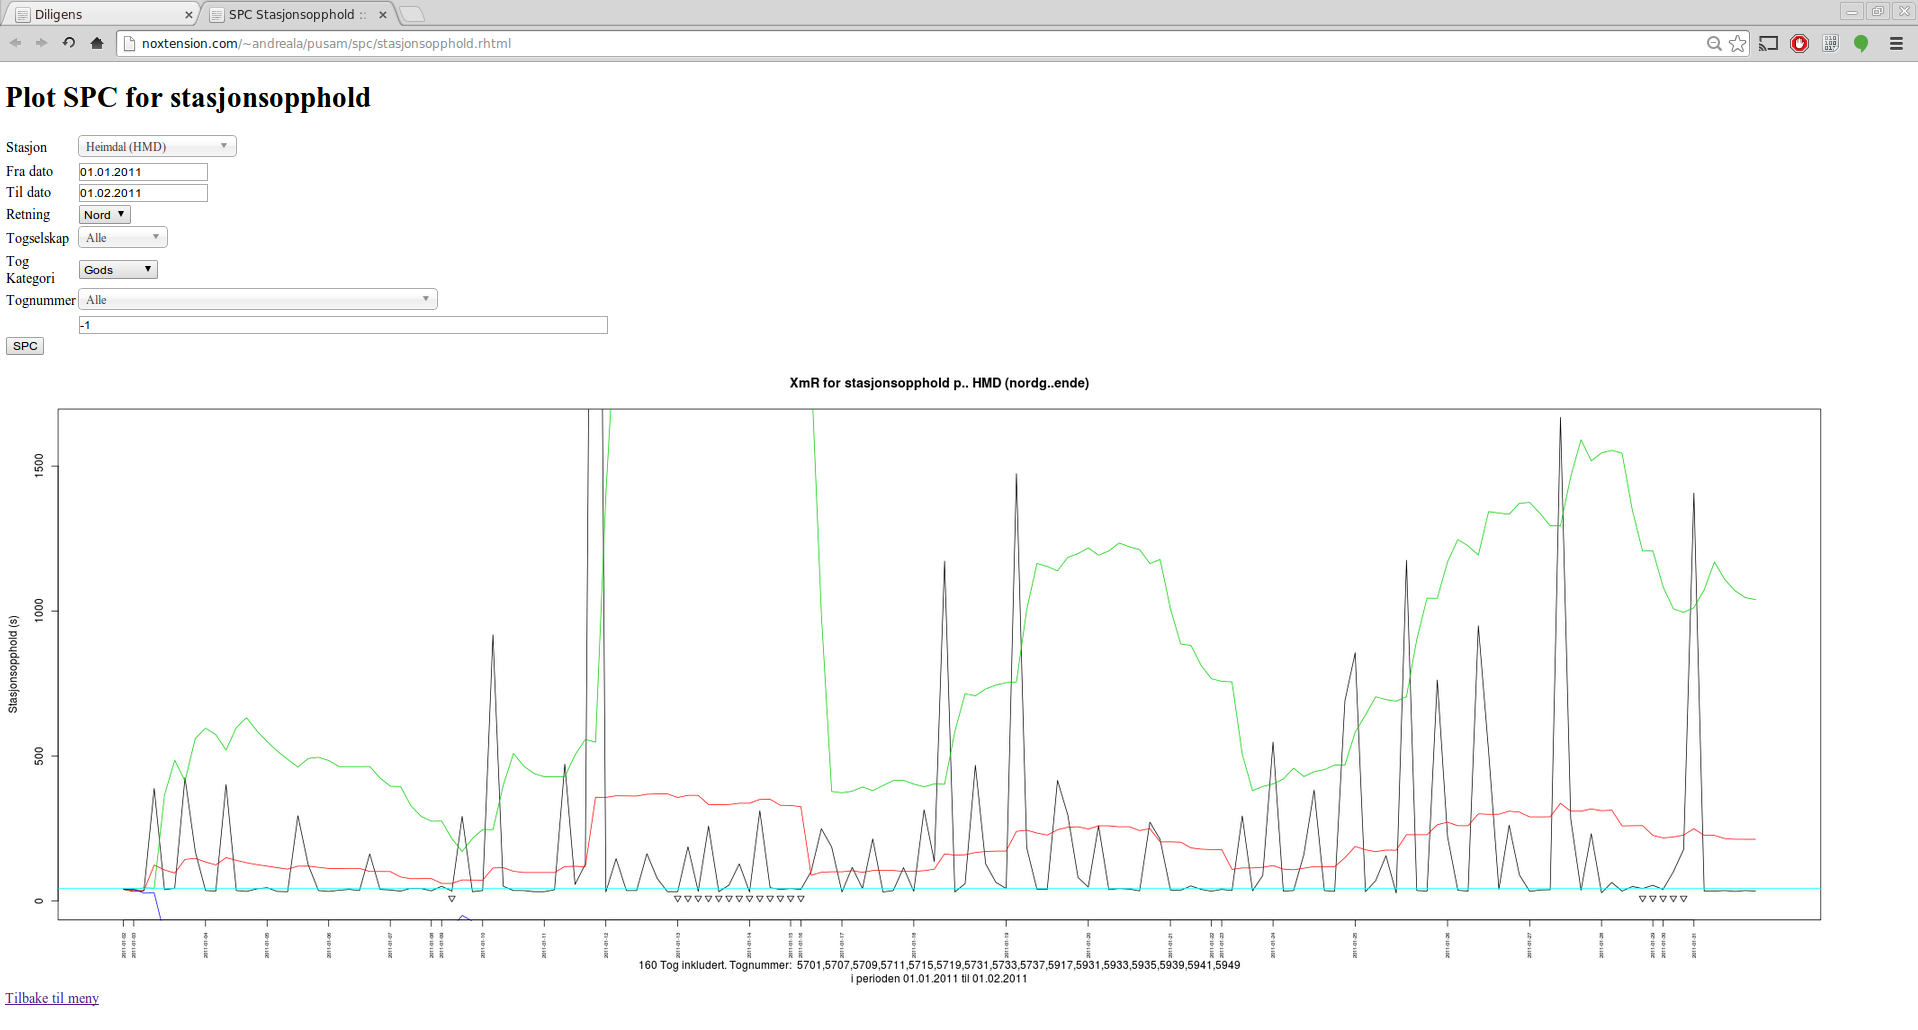
\includegraphics[width=\textwidth,center]{plot-spc-stasjonsopphold.png}
	\caption[Time at station (SPC)]{Time at station (SPC) \cite{sintefPresis}}
	\label{fig:plot-spc-for-stasjonsopphold}
\end{figure}
\pagebreak

\begin{figure}[!htbp]
	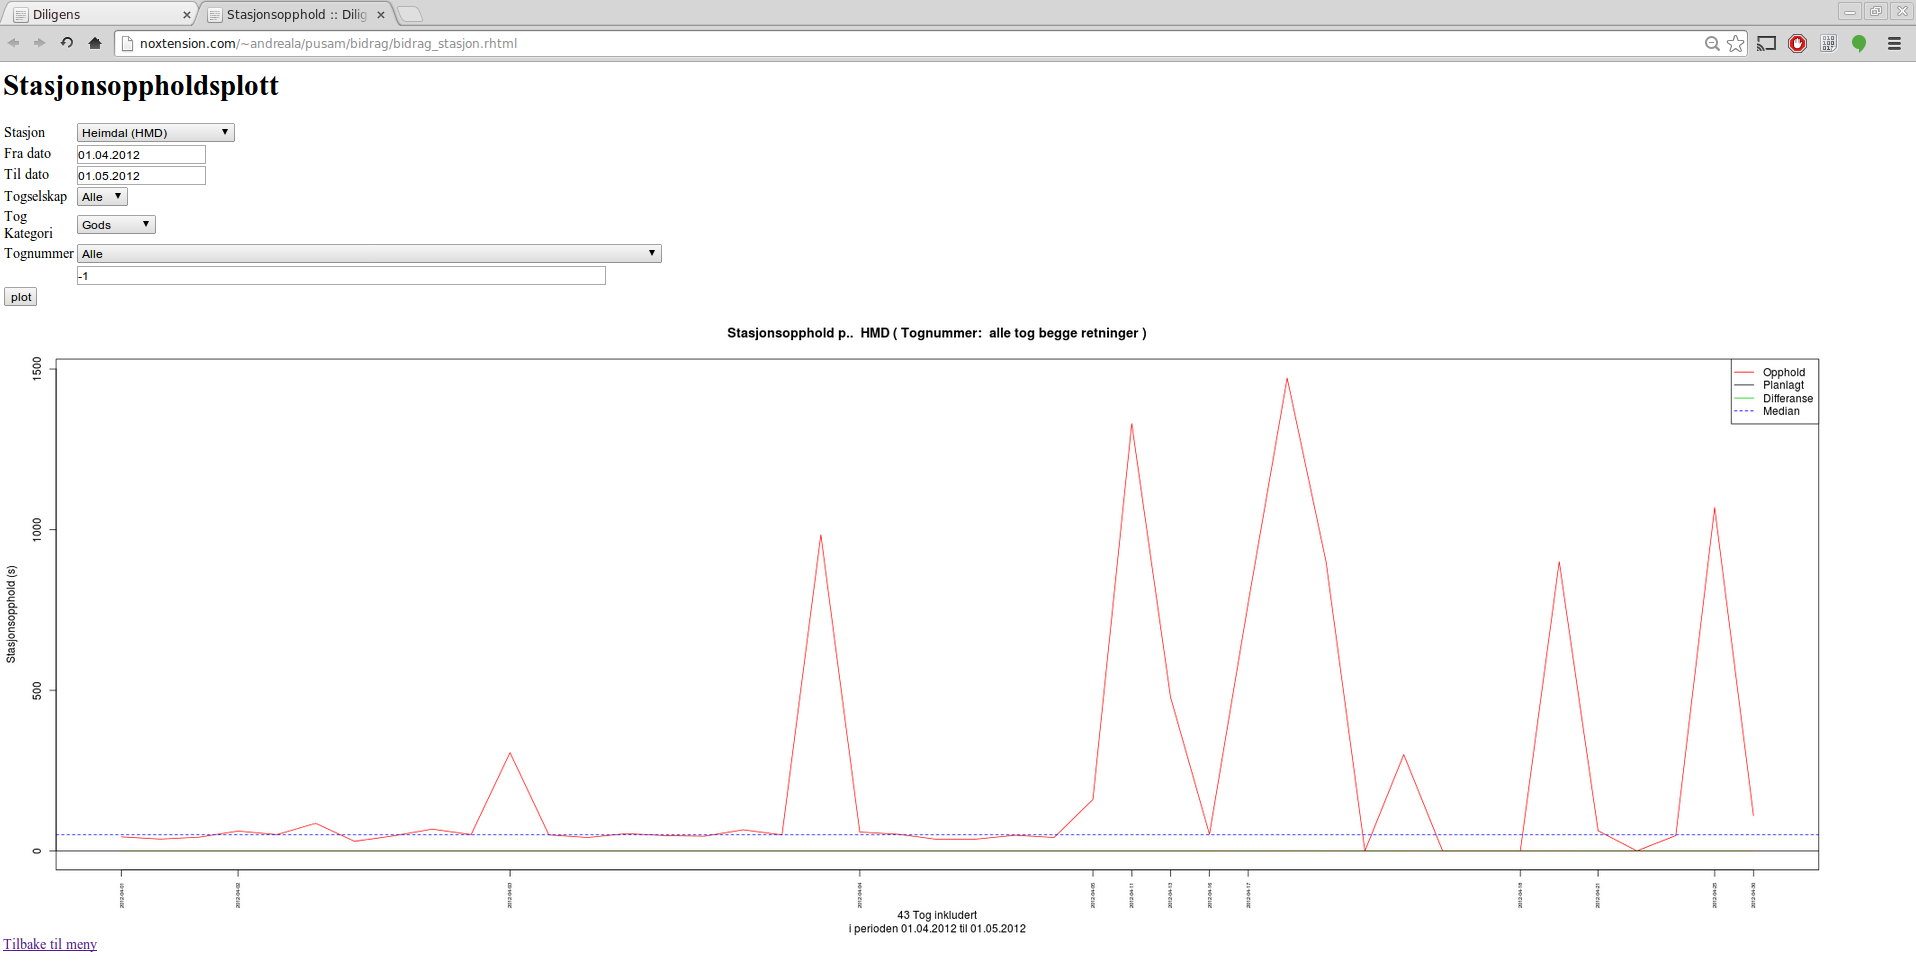
\includegraphics[width=\textwidth,center]{stasjonsoppholdplott.png}
	\caption[Time at station (Bidrag)]{Time at station (Bidrag) \cite{sintefPresis}}
	\label{fig:stasjonsoppholdplott}
\end{figure}
\pagebreak

\begin{figure}[!htbp]
	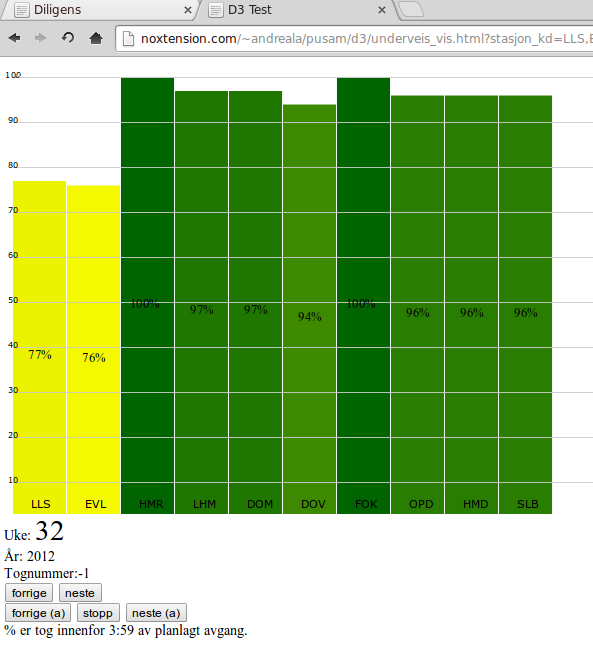
\includegraphics[width=\textwidth,center]{ukespunklighet.png}
	\caption[Weekly punctuality between stations]{Weekly punctuality between stations \cite{sintefPresis}}
	\label{fig:ukespunklighet}
\end{figure}
\pagebreak

\clearpage
\subsection{Cargonet} % (fold)
\label{sub:subsection_cargonet}

% subsection subsection_name (end)
Cargonet is a Norwegian which provides intermodal transport on rails. To 
provide a effective tracking service for the customers, Cargonet provides a 
internal service for the users which tracks all trains belonging to Cargonet.
As can be seen on \vref{fig:cargonet}, it only shows a picture of the current
status of each train, it lacks the possibility to analyze both each stretch 
individually  and analyze trains and stretches in time.

\begin{figure}[!htbp]
	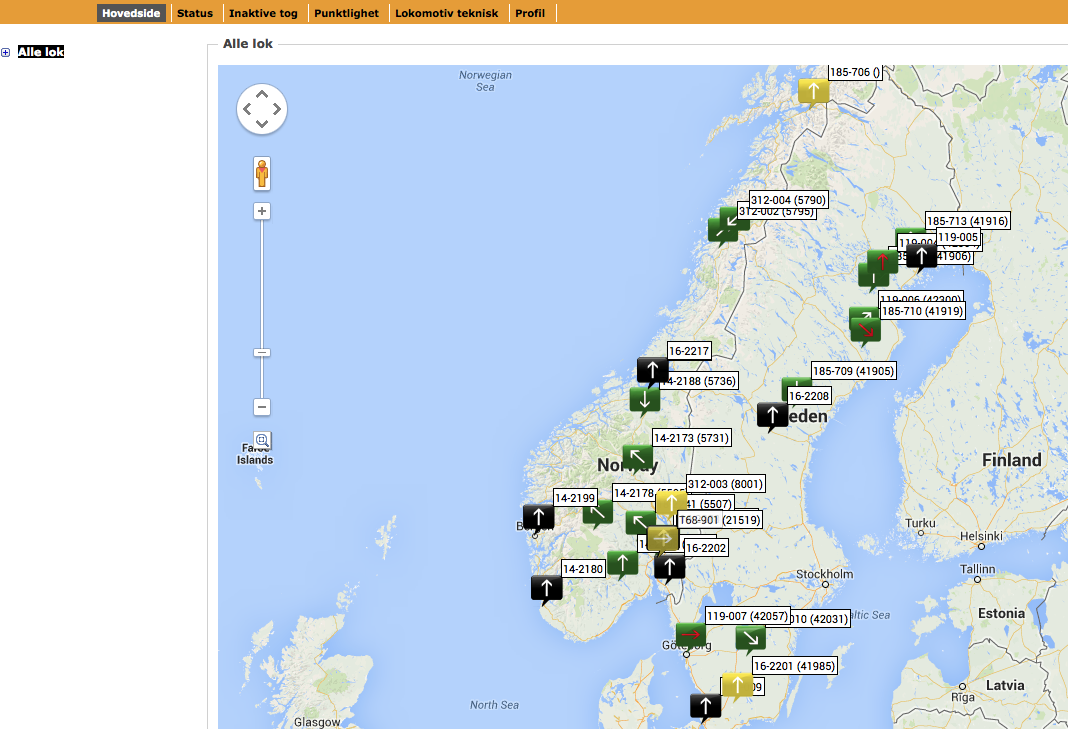
\includegraphics[width=\textwidth,center]{cargonet.png}
	\caption[Cargonet]{Cargonet \cite{cargonet}}
	\label{fig:cargonet}
\end{figure}

\begin{itemize}
	\item Red arrow:\hspace{4ex} Delayed.
	\item White arrow:\hspace{4ex} On time.
	\item Red box:\hspace{4ex} Locomotive driven 2km without carriages.
	\item Black box:\hspace{4ex} Locomotive without carriages.
	\item Yellow box:\hspace{4ex} Locomotive on time without schedule, or known position.
\end{itemize}

\pagebreak
% subsection subsection_cargonet (end)
 % and state of the art
%% !TEX root=../thesis.tex
\chapter{Method}
\label{chapter:method}

In working with this project the group has undertaken a considerable study of
literature around both software architecture, software metrics and assessment, electronics, display technology,
and studies about driver environments and performance. The literature has
served as a platform to support our project goals of creating an enabling
software architecture. The group has also conducted an interview with a driver
from last years Revolve-team. In collaboration with Revolve we have elicited
requirements and use-case scenarios which in turn has resulted in our proposed
architecture design (including design artifacts) and assessment guidelines.

The biggest weakness of the architecture described herein is the lack of
verification. First, during the project period we didn't have access to any hardware
similar to the one the system will be running on. Second, there are still some
uncertainties with regards to the amount of data that is to be handled by the
system due to the fact that sensor update rates and CAN-bus package format is
still an unknown factor. We have however developed a proof-of-concept desktop
application to simulate a configuration environment for the proposed system.
We will be discussing this application further in \vref{chapter:results}. 

\section{Literature Study}
To acquire a broad picture of the problem area and domain the group has studied
a varied set of literature ranging from research articles to books on various topics. Some of the most useful literature we have read includes the following:
\begin{itemize}
	\item ``An Introduction to Object-Oriented Analysis and Design and Iterative Development'' by Craig Larman \cite{Larman:UML}
	\item ``Software Architecture in Practice'' by Bass, L. and Clements, P. and Kazman, R.
	 \cite{bass2012software}
	\item ``Designing embedded hardware [Kindle Edition]'' by John Catsoulis
	\item ``A software architecture evaluation model'' by Dueñas, Juan C and de Oliveira, William L and Juan, A.
	\cite{duenas1998software}
\end{itemize} 
For an exhaustive list of all literature used we refer to the
bibliography\vpageref{bibliography}.

\section{Architecture Design Method}
In the process of designing this architecture we have opted to use design
artifacts and methods described by Craig Larman \cite{Larman:UML}. We started
out at the beginning with performing an interview with one of last years 
drivers (\vref{interview:bakkom}) to get a picture of how the cockpit 
experience is for the driver during
an event. We also got some interesting ideas to build on. Building on this
information we arranged an informal requirements workshop together with a few 
members of this years Revolve-team; eliciting both quality requirements and
functional requirements (and lots of ambitious ideas). One important benefit of
bringing experienced members in on the workshop was that we could easily
discover external requirements originating in the FS competition rules \cite{fsae:2014rules}.
Both Larman and Bass et al. suggests that a systems
architecture should be based mostly on non-functional and quality requirements,
especially those that strongly influence the architecture.
\cite[p.20]{bass2012software}\cite[pp. 541-554]{Larman:UML}

After the workshop we started working on refining and defining the results,
writing up use-cases in a terse format. Larman suggests \cite[pp. 95-95]{Larman:UML}
that during early phases of development most use cases (except the ones that 
might be architecturally significant or with high risk) should be kept terse 
and rather be expanded upon and refined when development is underway. Since no
architectural development was performed during this project we decided to spend
more time trying to clarify them and use the results to help with identifying
the architectural requirements.

In the further process we listed the discovered requirements in an
architectural factors table \cite[pp. 56-59, 545-547]{Larman:UML}. The goal of
this activity was to define measures that can be used to measure the
architecture's ability to meet the goals and requirements, and to give an
easily accessible ranking of importance for these requirements.

The last artifact to be developed was the system architecture document \cite[p. 550]{Larman:UML} where we
recorded and detailed the suggested solutions, and their reasoning, to resolve the architectural
factors.

In working with the architecture design we have tried to work in an iterative
fashion, but due to the compact nature of the project some processes bear the
look and feel of a ``waterfall'' process. We do not intend that the
architectural design suggestion presented in this project to be the final one, 
but rather its intended to be a good
starting point for development and refinement. We also suggest metrics that can
be used to measure if the architecture meets the goals set, and believe it is important
that the control process starts early in the development to see if the
architecture meets the requirements or needs further work 
\cite[pp. 556-557]{Larman:UML}.

In describing our architecture we have opted to use UML, or modeling close to
UML where we felt that it increased readability, or where we were pressed for time and
UML compliance wasn't deemed the most important, planning to revise this when
further development is being undertaken. We chose to not use any ADLs to describe the
system, in part because that would be worthy a project of its own, and in part because we 
are not interested in traces of the system 
\cite[p. 42-43]{Roscoe:2005:TPC:550448},
but in the systems ability to meet its critical requirements. 




%% !TEX root=../thesis.tex

\chapter{Results}
\label{chapter:results}
This chapter will present results found by performing activities described in
\Ref{cha:research_questions_and_method} \nameref{cha:research_questions_and_method}. 

In the two first parts we describe the results of the workshops held. The last 
part describes the functionality in the prototype developed. The implementation
of the prototype was described in \Ref{cha:implementation} \nameref{cha:implementation}.

% !TEX root=../../thesis.tex

\section{Workshop 2014-04-04} % (fold)
\label{sec:workshop_2014_04_04}
The first workshops agenda was to help define the stakeholders of the system,
their areas of responsibility, and their needs. The workshop was also meant to 
bring clarity to how the system will relate to these users and their needs.
Attending this workshop was Andreas Amdal Seim (SINTEF), Andreas Dypvik 
Landmark (SINTEF), Rimmert van der Kooij (SINTEF), Nils Olsson (NTNU), Per 
Magnus Hegglund (Jernbaneverket), Magnus Bae (NTNU), and Magnus Krane (NTNU).\\

Perspectives that can be used when viewing the system were discussed
first.
\begin{itemize}
	\item Infrastructur: Segment director, etc.
	\item Traffic division / passenger / train companies.
	\item Delay causes: delay demographic.
\end{itemize}

Interests of users when using the system were then discussed based on the
perspectives.
\begin{itemize}
	\item Uptime, punctuality.
	\item Deviation.
	\begin{itemize}
		\item What?
		\item Where?
		\item When?
	\end{itemize}
	\item Delay time.
	\item Variation.
	\item Changes.
\end{itemize}

Causes that might affect the punctuality was also listed: weather, number of
passengers, capacity utilization, animal accidents, cargo volume.
The causes was concluded not to be included in this project, as the causes is
difficult to prove and get data on.\\

The internal project in Jernbaneverket (section
\Ref{sub:subsection_jernbaneverket}) uses a deviation registry for data to
analyze each stretch on a detail level. To calculate the uptime, presented in
\Ref{sec:railway_operations}, also uses the deviation registry for the needed
data. A problem by using the deviation registry for calculating variation or 
changes, the registry have a five minute filter in which the trains are being 
calculated to be on time.

Two problems were agreed upon that needed to be addressed, the back end and 
the  front end of the system. What kind of data is available and what is 
possible to do with this data? A data set can show both positive and negative 
results, based on what the set are compared too. For instance, easter is not 
on the same week each year and the passenger volume increase during the 
holidays. Data sets ended up being addressed in the second workshop (\Ref{sec:workshop_2014_04_24}). 

As the different stakeholders might have need for different presentation of the
data, different levels of stakeholders and what should be shown in each level 
was discussed. A suggestion was made to have the same perspective through the
levels, but to have selectable views based on roles. \\

At the end of the workshop, three conclusions was made. The first conclusion 
was to have a dashboard next to each marker with relevant data to the current 
stakeholder. The second conclusion was to a interactive list of the
stakeholders which adapted the visual presentation to the selected stakeholder,
presented in \Ref{sec:back_stakeholders}.
The last conclusion was to have a second workshop where the content of the
dashboard should be decided. This resulted in \Ref{sec:workshop_2014_04_24}.

% section workshop_2014_04_04 (end)

\section{Workshop 2014-04-24} % (fold)
\label{sec:workshop_2014_04_24}
The second workshops agenda was to determine what statistical data was 
to be implemented in the dashboard, concluded upon in \Ref{sec:workshop_2014_04_04}.
Attending this workshop was Andreas Amdal Seim (SINTEF), Andreas Dypvik 
Landmark (SINTEF), Rimmert van der Kooij (SINTEF), and Magnus Krane (NTNU).\\

The workshop started with a brainstorming for different data to present in
the map. The different data was ranked on implementation practicality from 1 - 
3 where 1 is unpractical and 3 is very practical; and ranked on the 
desirability of the data from 1 - 3 where 1 is undesirable and 3 is very 
desirable. The brainstorming after ranking is presented in \Ref{table:dashboard_functionality_wants_vs_needs}.
\\

\begin{table}[!h]\small
	\begin{tabularx}{\textwidth}{|X|l|l|l|}
		\hline
		Functionality & Practicability & Desirable & Priority\\
		\hline
		Outstanding errors & 1 & 1 & 1\\
		\hline
		Suspensions & 3 & 1 & 3\\
		\hline
		Variation & 1 & 3 & 3\\
		\hline
		Season effects & 3 & 1 & 3\\
		\hline
		Follow delays & 1 & 3 & 3\\
		\hline
		Speed limits & 3 & 1 & 3\\
		\hline
		Cause & 3 & 2 & 6\\
		\hline
	 	Worst stretch/station/train number & 3 & 2 & 6\\
		\hline
		Traffic density & 3 & 3 & 9\\
		\hline
		Speed restrictions & 3 & 3 & 9\\
		\hline
		Delays & 3 & 3 & 9\\
		\hline
		Crossings & 3 & 3 & 9\\
		\hline
	\end{tabularx}
\caption{Dashboard functionality brainstorming ideas}
\label{table:dashboard_functionality_wants_vs_needs}
\end{table}

Based on the ranking, the decision was made to only implement the data was
ranked as a 3 both on practicability and desirability, presented in the list
below.

\begin{itemize}
  \item Delays
  \item Speed restrictions
  \item Crossings
  \item Traffic density
\end{itemize}

The second part of the agenda, was to determine how the selected data was to be
presented. The decision was made to split the presentation in two parts. The
first was to display aggregated data in the dashboards next to the marker based
on the current stakeholder. The second was to display top 5 lists for delays
and speed restrictions.

\subsection{Crossings} % (fold)
\label{sub:crossings}
One of the problems discussed with crossing was should the system take into 
account the difference between actual crossings and planed crossings or not? 
The difference is hard to calculate as one does not know whether one of the 
trains involved in the planned crossing, was canceled or just delayed. The 
decision was made to present the number of crossings occurred at each station, 
and aggregate the number as one navigates in the stakeholder hierarchy.
%TODO planned crossings, ask Landmark.
% subsection crossings (end)

\subsection{Traffic density} % (fold)
\label{sub:traffic_density}
Several options to present traffic density were discussed, the problem was how
to correctly show the number of trains based on the data available. 
Should the system present each train based on the train numbers and 
calculate for the entire line both ways? Should the system display train 
numbers divided by the segment directors? 

In the workshop it was decided to show the number of trains that passes each 
block segment, based on the data available. When navigating in the hierarchy,
the system shall aggregate the number of trains.

% subsection traffic_density (end)

\subsection{Speed restrictions} % (fold)
\label{sub:speed_restrictions}
Speed restrictions was decided to be presented a marker per restriction, and be
shown between the selected time interval. The data for the speed restrictions
was to be presented in a plot which appeared in the marker for each
restriction.

%In the dashboard it was decided to show the top 5 upper and lower bounds. It was also decided to include a little marker on the map to indicate the location of the speed restriction. 

% subsection speed_restrictions (end)

%\subsection{Delays} % (fold)
%\label{sub:delays}
%TODO
%Since delays can cover a large area depending on how you define it, this had to be properly discussed and defined. Should you follow the Norwegian standard \cite{jernbaneverketPunklighetsTall} of only say that a train is delayed at the final destination or use data from the signal post on the stretches  compared to the schedule? Should you take the variation into account? It was decided to display the sum of the seconds the of delays, and sum of trains arriving to early. These sums would then be displayed in the dashboard and be aggregated according to the level.

% subsection delays (end)

% section workshop_2014_04_245 (end)

% section workshops (end)

% !TEX root=../../thesis.tex

\section{Prototype functionality} % (fold)
\label{sec:prototype_functionality}
As part of answering the research question, a prototype was developed. In this
section we will describe the functionality in the prototype.\\

The prototype is a map based system that presents the information according to
the needs of the stakeholders, as presented in \Ref{fig:map_prototype}. A
intractable list was implemented, presented in \Ref{fig:stakeholder_selection_list},
which gives the functionality to navigate through the stakeholders hierarchy.
The system aggregates the data according to the current selected stakeholder,
as presented in \Vref{sub:back_end_aggregation}. The visual presentation will 
be adapted to the the areas of responsibility of the current stakeholder, 
which will focus the presentation of the data in the geographical area of the 
stakeholder.

To let the stakeholder be able to select different types of information
according to their need, a intractable list was implemented (\Ref{fig:implementation_type_selection}).
By letting the user select the information type to present, the system is able
to present the stakeholders need for different information type according to
their requirements. \Ref{fig:crossings_and_speed_restriction_implementation}
shows the presentation of two different types of information.\\

A method to navigate in time were implemented, as the stakeholders have 
different needs for the level of detail in the presentation of data. The time
navigation were implemented as two input boxes, see \Ref{fig:time_selection_implemented}.
The system uses the time interval set by the user to limit the data to be
processed. 

\begin{figure}[!htbp]
	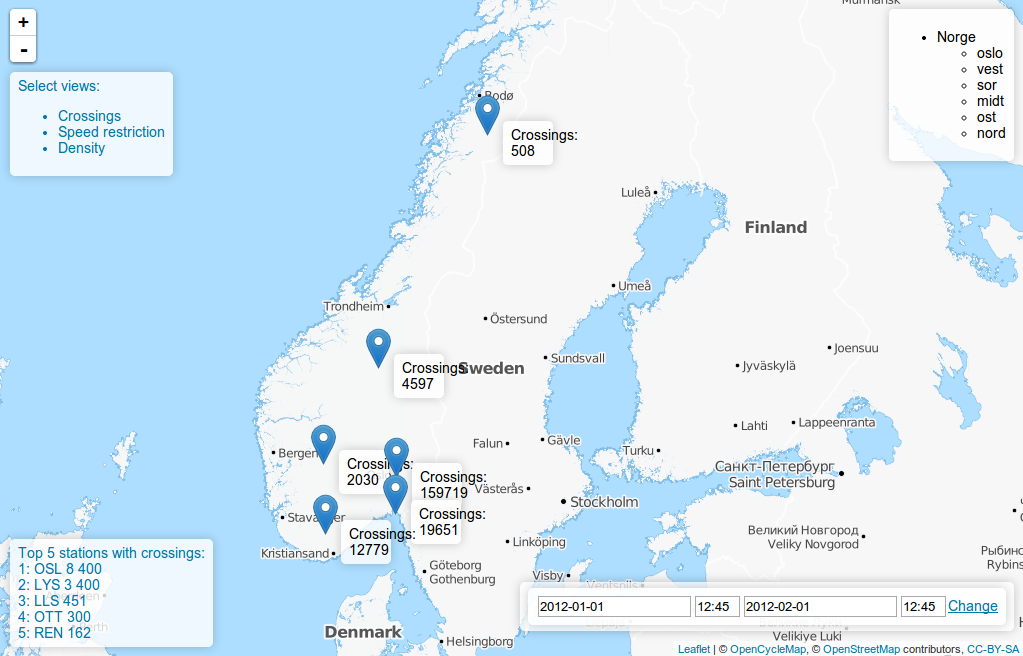
\includegraphics[width=\textwidth,center]{map_prototype.png}
	\caption[Map implementation]{Map implementation}
	\label{fig:map_prototype}
\end{figure}

\begin{figure}[h!tbp]
	\centering
	\begin{subfigure}{0.4\textwidth}
		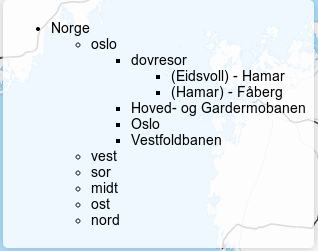
\includegraphics[width=\textwidth]{stakeholder_selection_list.png}
		\caption[Stakeholder selection list]{Stakeholder selection list}
		\label{fig:stakeholder_selection_list}
	\end{subfigure}
	\begin{subfigure}{0.3\textwidth}
		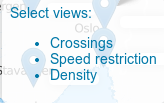
\includegraphics[width=\textwidth]{information_type_selection.png}
		\caption[Information type selection]{Information type selection}
		\label{fig:implementation_type_selection}
	\end{subfigure}
	\caption[Stakeholder selection and Information type]{Stakeholder selection and Information type}
	\label{fig:stakeholder_selection_and_information_type}
\end{figure}

\begin{figure}[h!tbp]
	\centering
	\begin{subfigure}{0.4\textwidth}
		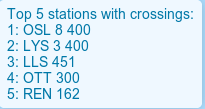
\includegraphics[width=\textwidth]{top5.png}
		\caption[Top 5 list]{Top 5 list}
		\label{fig:top_5_list}
	\end{subfigure}
	\begin{subfigure}{0.6\textwidth}
		
\includegraphics[width=\textwidth]{time_selection_implemented.png}
		\caption[Time selection implementation]{Time selection implementation}
		\label{fig:time_selection_implemented}
	\end{subfigure}
	\caption[Top 5 list and Time selection]{Top 5 list and Time selection}
	\label{fig:Top5_list_and_time_selection}
\end{figure}

\begin{figure}[h!tbp]
	\centering
	\begin{subfigure}{0.6\textwidth}
		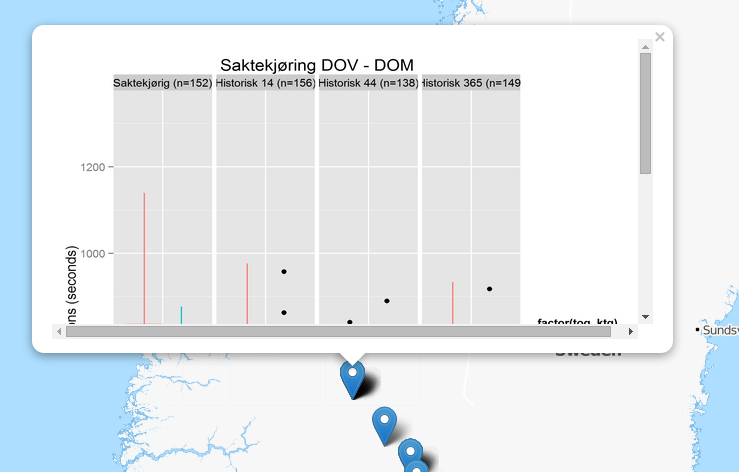
\includegraphics[width=\textwidth]{speed_restriction_presentation.png}
		\caption[Speed restriction presentation]{Speed restriction presentation}
		\label{fig:speed_restriction_presentation}
	\end{subfigure}
	\begin{subfigure}{0.25\textwidth}
		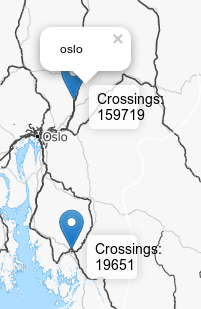
\includegraphics[width=\textwidth]{crossings_presentation.png}
		\caption[Crossings presentation]{Crossings presentation}
		\label{fig:crossings_presentation}
	\end{subfigure}
	\caption[Speed restriction and Crossings implementation]{Speed restriction and Crossings implementation}
	\label{fig:crossings_and_speed_restriction_implementation}
\end{figure}

% section prototype_functionality (end)


%% !TEX root=../thesis.tex
\chapter{Discussion}
\label{chapter:discussion}

\section{Stakeholders and aggregation} % (fold)
\label{sec:discussion_stakeholders'_and_aggregation}
It is important to define the needs and requirements of the stakeholders 
early in the process, in order to design a system that gives the right scope. 
By the aid of workshops we defined the requirements, as it is part of the 
research method (see \Ref{sec:workshops}). We can define the stakeholders in 
a hierarchy, based on their organizational structure, and areas of 
responsibility, this aids us in defining the requirements on the structure of 
the information presented.

There is a good synergy between the requirements and the system, when the 
system is designed with the stakeholders' wishes for viewing different type of 
information in mind. The synergy between the requirements and the system has 
both advantages and disadvantages. On one side the system has a great 
possibility to satisfy the requirements and needs of the stakeholders, since 
the system is tightly connected to the requirements. On the other side, the 
system can be inflexible to large changes, if the requirements change late in 
the project. In the workshops, we defined that the stakeholders must have the 
ability to view different kinds of information; the system must take these 
needs into consideration. A system capable of supporting a providing 
“awareness in presentation” of multiple stakeholders is by the very nature 
more complex. Such a system would have to process a larger amount of data than 
a single-perspective system in order to provide the required functionality. 
Processing larger amounts of data leads to a more complex system (back-end) – 
and in turn a more complex interplay between user and front-end, with effects 
on the interplay between front-end and back-end. The system can be more 
dynamic by reusing parts of the data processing for 
different information types, when designed with the needs as well as the 
requirements in mind. In order to meet the requirements of the different 
stakeholders needs we have to aggregate data. There are several ways to 
aggregate the groups of data according to the given criteria. The method used 
for aggregation of data that enables the best view for the stakeholders is not 
straightforward. We have chosen to explore the following simple alternatives: 
average, minimum, maximum, median, and frequency (count). These are by no 
means an exhaustive list, but represent well established, robust and simple to 
implement alternatives. To decide the aggregation method, we have to consider 
how each information type is structured, but also how this structure fits in 
with the stakeholder and their hierarchy. During the workshops, we decided 
that the way to aggregate the data that was best suited to the requirements is 
to take the average; the decision was based on how the data is connected to the stakeholders and their hierarchy.

When returning the processed data to the user, the system can use the 
context of the various stakeholders to aggregate the presentation of the data. Since the stakeholder hierarchy contains the area of responsibility of each stakeholder, the system can fit the visual display to the step of the current stakeholder. The system uses processed data for aggregating the hierarchy to find the stakeholder. Fitting the view to the stakeholder provides detail for a single stakeholder; this is useful for presenting a single stakeholder and their step.
%To let the user decide the detail level of the display can be useful, since the display then has the opportunity to present more overall information. 
We decided to fit the visual presentation of data 
to the current stakeholder, and have the opportunity to jump, back and forth, 
within the hierarchy of the stakeholders. By fitting the view to the 
stakeholder, the display enabled the user to receive more relevant information 
on the current stakeholder. A conflict of interest occurs between stakeholders 
due to overlapping areas of responsibility. The conflict is extremely difficult 
to consider, and is not taken into consideration when aggregating the data or 
fitting the view.

As the area director wants to study data from the entire area for a large 
period of time, and the segment director wants to study almost every detail 
that occurs on the segment, manual navigating in time was decided to use as a 
way to increase and decrease the level of detail in the data presented.

\subsection{Stakeholder and aggreation keywords} % (fold)
\label{sub:stakeholder_and_aggreation_keywords}
Keywords:

\begin{itemize}
	\item Important to define requirements early, in order to make an appropriate system, that is useful for the stakeholders'
	\item How to define the stakeholders' and requirements for use with a system?
	\begin{itemize}
		\item important to define who are the stakeholders'
		\item important to define what the stakeholders' needs are
		\item important to define to which need are connected to which stakeholder, in order to show the correct information in the system connected to each of the stakeholders' needs.
	\end{itemize}
	\item How can we design a system that used the requirements needed by the stakeholders' to process the data and visualize the data in such a way that the stakeholders' needs are met?
	In order to meet the requirements of the stakeholders' needs we need to aggregate the data. The following .....
	\item aggregation of data:
	\begin{itemize}
		\item two goals: geographic \& time
		\item aggregation based on detail level of visualization
		\begin{itemize}
			\item based on stakeholders' need
			\begin{itemize}
				\item detail level in map
				\item which area is shown in the map
				\item aggregation based on time
			\end{itemize}
		\end{itemize}
	\end{itemize}
	\item Data aggregation methods
	\begin{itemize}
		\item What are good ways to aggregate the data?
		\item How to determine what fits the requirements?
	\end{itemize}
	\item How to present the data to the users based on the requirements? (detail
	level per stakeholder in the hierarchy)
	\item Time navigation for zooming through the data.
\end{itemize}

% subsection stakeholder_and_aggreation_keywords (end)


% section stakeholders'_and_aggregation (end)

\section{Data storage and data queries} % (fold)
\label{sec:discussion_data_storage_and_data_queries}
As the data sets originate from different sources and contain different
structures, they can be difficult to efficiently query if not structured
correctly. One option for the structure is to merge all the
data sets into one large database, by merging the data sets in one large
database, the data are structured in an client-server architecture. 
A client can either communicate to the databases directly or through a middle
tier. Three-tier architecture is a very common solution on the Internet, where 
the communication between the client and the database goes through a service 
layer \cite[pp. 294-297]{toftHanseMallaugDatabaser}. The client-server 
architecture has the benefits of giving the front-end applications a single 
point of connection, avoiding duplication of data, and giving the database 
manager both a single structure to maintain and a single point of access with 
easier access control.

The alternative of the client-server architecture is a distributed
database \cite[pp. 301-303]{toftHanseMallaugDatabaser}. The distributed database
architecture is done by splitting the storage of data and the processing of
data over several servers. Some benefits of the distributed architecture are 
easier expansion, modular sets with built-inn flexibility, and if one node 
goes down the others still work. Exercising the built-inn flexibility of each
module is usually cheaper than to hand-code a specific change in hindsight\cite[pp. 117-130]{Bass:2012:SAP:2392670}. The distributed architecture is a 
modifiable data storage, where the modular sets are loosely linked sets. 
%software architecture p. 185 for other quality attributes
We demonstrated a hybrid of the client-server and distributed
architecture \cite[pp. 297-299]{toftHanseMallaugDatabaser}.

By using the three-tier architecture, we implemented a middle-tier which 
processed the data, and a lower tier containing several databases, see \Ref{fig:three-tier_architecture}. For
structuring the data sets with the stakeholders' requirements in mind, we
utilized one database which contained the stakeholders' areas of responsibility in
their hierarchy, and each of the other databases for different types of 
information. The semi-distributed databases mean that it is easy to remove or
add data sets, since the different types of information are connected to the
stakeholders' hierarchy. There are also some negative aspects using
the semi-distributed databases, for example: some data fields
will be duplicated. The duplication of data will lead to redundancy and
increased probability for data corruption and errors. In our case the duplication can be found as stations in the databases, due to the stations acting as the
connection between every data set. In the three-tier, distributed database, 
and semi-distributed architecture, the data have to be processed from the 
original source to fit in with the data structure.\\

We can increase the responsiveness of the system by utilizing the back-end for 
processing the data, since it usually on the same hardware as the databases or 
same sub-net, which provides quicker calls and responses to the databases from 
the data processing methods. As the aggregation averages the data based on the variables selected by the user, the data transferred from the back-end to the front-end will be reduced. Having a reduced amount of data to transfer, means that the system will experience quicker communication times. We 
have no control over what hardware the end user has, while the back-end 
is usually dedicated to one service and we can (more easily) control, and if 
necessary upgrade, the hardware.

The amount of data to be processed by the system is affected by three 
variables. The affecting variables are the stakeholders' need to navigate in 
time, the navigating in the stakeholder hierarchy, and the type of information.
As the level of detail increases by navigating in time, the amount of data to 
process decreases. Similarly by decreasing the level of detail, the amount of 
data to process increases. The navigation in the hierarchy affects the amount 
of data, as the further up in the hierarchy one navigates, the larger the 
areas of responsibility grows. The information type affects the amount of data 
in a data-set, because each information type have different needs for the 
amount of data to be processed. The system performance is determined by the 
amount of data to process, as it uses more time to process more data. 

\subsection{Data storage and data queries keywords} % (fold)
\label{sub:data_storage_and_data_queries_keywords}
Keywords:
\begin{itemize}
	\item Data set structure in prototype
	\begin{itemize}
		\item How should the data sets be structured when the sets are based 
		on the stakeholders' need for different type of information?
		\begin{itemize}
			\item Connection to the requirements of the stakeholders'.
			\begin{itemize}
				\item Stakeholder responsibility area from the hierarchy
			\end{itemize}
			\item Advantages and disadvantages with one or several sets in storage.
			\begin{itemize}
				\item Scalability and modifiability ref quality attributes \cite{Bass:2012:SAP:2392670}
				\item Duplication of data with several sets of data.
			\end{itemize}
		\end{itemize}
	\end{itemize}
	\item Data queries
	\begin{itemize}
		\item Limit queries for data processing efficiency 
		and more responsive systems
		\begin{itemize}
			\item By the aid of time navigation and requirements, limit the 
			queries for more efficient calls to the data storage.
			\item The system will be more efficient in the processing of the 
			data, when limiting the quires.
		\end{itemize}
		\item Front end vs back end data processing for system efficiency and
		limiting data traffic
		\item Should the data be processed in the front-end or the back-end 
		of the system?
		\begin{itemize}
			\item The data should be aggregated in the back-end of the system, 
			since it is more efficient.
			\begin{itemize}
				\item Quicker calls to the database from the back-end.
				\item Less data traffic during transfer of.
				\item Usually quick hardware on server side, while it have a 
				great span in the front-end.
			\end{itemize}
		\end{itemize}
	\end{itemize}
\end{itemize}

% subsection data_storage_and_data_queries_keywords (end)

% section data_storage_and_queries (end)

%\section{Review of own work} % (fold)
%\label{sec:review_of_own_work}
%Keywords:
%\begin{itemize}
%	\item Appropriate method?
%	\item 
%\end{itemize}
% section review_of_own_work (end)

%% !TEX root=../thesis.tex
\chapter{Conclusion and future work}
\label{chapter:conclusion}


\label{bibliography}
\bibliography{bibliography}
%\nocite{*} %All
%\nocite{key1,key2,keyN}

%Use ieeetr to get correct numbering of references according to the IEEE
% standard. Numbering follows order of introduction.
\bibliographystyle{ieeetr}


% Header for appendices
%\chapter{Appendices}
%    \begin{center}
%    \topskip0pt
%    \vspace*{\fill}
%     This page intentionally left blank     %   Nice and centered :D
%    \vspace*{\fill}
%    \end{center}

%\appendix
%\setcounter{page}{0}
%\pagenumbering{roman}
%% !TEX root=../thesis.tex

\chapter{Theory}

In this appendix we look at --- meh!

\subsection{Types of systems}
In general there are basically two types of driver information systems, Heads Down Display and Heads Up Display. 
The first is represented by the classic we all know; the dashboard. The second we find in more advanced 
applications such as in fighter planes where the pilot wears a helmet with a display in the visor. In the latter 
example the operator has a display that is fixed in position, but because the helmet moves with head movement, so does
the display. In the first example the display is fixed and operator head and eye movement is required to use the display during normal
operation.

Revolve have always chosen to utilize dashboard-based information systems. Mainly consisting of LED-displays and 
LED-indicators. To get an insight into the efficiency of these systems we conducted an interview with a driver 
from the 2013-competitions. During this interview we learned that during a race it is very hard to consume
information from the dashboard. The course twists and turns, and requires the driver to focus on track and on handling the car; braking and 
acceleration. This makes it difficult for the driver to shift focus down to the dashboard and usually requires longer straight sections of
track to be able to gather any meaningful information.



% \subsection{Scope}
% The scope of this project is to research the state-of-the-art of 
% HUD-technology. What type of devices and technology that can 
% be leveraged to create a prototype HUD for application in a racing car. 
% Focusing both on the racing parts of the competition, and on helping
% to win points in the business side of the competition. (link to background chapters)

% \subsection{Application}Incorporating a HUD-system in a race car is something that could provide a competetive advantage. For Revolve NTNU 
% this is doubly so, since the Formula Student competetion covers so many disiplines the advantages given may also contribute to better 
% results in business-class competitions. (link to background chapter here)
 %maybe we should find something useful to put here
% before we include it ^^

%\addtocontents{toc}{\protect\setcounter{tocdepth}{0}}

%\chapter{Interviews}
\clearpage

\section*{Driver interview}
\label{interview:bakkom}
Date: 2013-09-25\\
Subject: Ole Edvard Bakkom\\
Interviewers: Magnus Krane and Magnus Bae\\
\\
The purpose of of this interview was two-fold: (1) To gain knowledge about what types
of information that a Formula Student class racecar-driver consumes during typical events 
under an FS-competion. (2) To discuss what type of information that would be feasible for the driver
to consume in different circumstances; racing, training, renting a high performance vehicle for a limited time.


\begin{dialogue}
    \speak{Magnus} During a race how much information do you manage to consume from the instrument panel? 
    \speak{Ole} Not much, maybe a blinking LED or two, but it's difficult to read the speedometer for instance. 
    	The pace is quite high, and very few straights. This makes it difficult to be able to look down
    	and focus on complex information. 
    \speak{Magnus} Do you think you'd be able to consume more information in competitive context if the information was 
    	presented in a way that you didn't have to shift your focus away from where you're looking, for instance a heads-up-display?
    \speak{Ole} Yes, I think that would be a considerable improvement over last year's solution, as long as it's not obtrusive.
    	Although the usage in the competition might be a bit limited, I think it could be amazing for testing.
    \speak{Magnus} How do you think it would contribute in testing?
    \speak{Ole} Well, there's lots of things, but the first that comes to mind is, since we're building an electric car this year,
    	charging level - to get a notification when the battery needs to be charged or battery percentage.\\
    	Second the ability to have two-way communication with the rest of the crew. Last year we had to stop whenever they wanted to
    	give a message.\\
    	Lap-times would definitively make a difference during testing. Previously we've had to wait until we switched drivers to get a list of our lap times.\\
    	Cone-hits, in the competition we get added times for every cone we hit(flip?), getting real-time or close to it feedback if we hit a cone would be very practical.
    \speak{Magnus} What about in the competition? Which of these would be important? Two-way communication maybe?
    \speak{Ole} In the competition we're not allowed to have two-way communication with the vehicle or driver. The vehicle is allowed to send, but not receive.
    	With reservations that they might have changed the rules for 2014.
    \speak{Magnus} So no two-way communication. Can you think of anything that could be valuable for the competion?
    \speak{Ole} Well, we're adding brake pressure adjustment, and showing data or settings for it could be very practical. Using data from wheel sensors
    	maybe you could show an alert if a wheel locks up as well, hinting the driver to adjust brake balance
    \speak{Magnus} Interesting, I'm automatically thinking Gran Turismo 5-style info. Basically graphics showing the four tires, and changing color to red
    	when one locks up.
    \speak{Ole} That could work. There's also been talk about monitoring tire temperature using infrared sensors.
    \speak{Magnus} There's also the business case; rental for the weekend-racing. What type of information do you think could be interesting in that
    	context, something that would sell well with the judges? We've been thinking about creating an optimal route for the track using GPS, and then showing deviance.
    \speak{Ole} That sounds like a good idea. How about showing ghost data? Best or last lap would be really cool. I think that would really make testing better too. 
    	If you could have a laptimer showing as well that would be a good motivator. 
    \speak{Magnus} Maybe having real-time difference between previous (or best) lap could work as well? And how about sectoring it, comparing on a corner-per-corner basis
    	 
    \speak{Ole} Definitely. If I could compare myself lap by lap I would definitely push myself harder. Trying out different racing lines and corner speeds would give 
    	instant feedback. That's something that I think would really be cool, both for training and the business case.\\
    	Using GPS-data, could you show optimal speed through a corner? If you know the layout of the track that could probably calculated? Alternatively comparing speeds through
    	corners with your own best speed. 
    \speak{Magnus} Interesting. Calculating theoretical optimum speed might be far from reality? How about giving achievments if your laptime is 13 seconds and 37 hundreds?
    	
    \speak{Ole} Hehe, achievments could be cool. Even if the calculated max speed is off you'd get an indication. If you go through a corner at 50 and max speed 
    	could be 70 it should mean that you can push harder.
    \speak{Magnus} Good point. How about drifting, showing you how far you drifted around a corner?
    \speak{Ole} The cars don't really drift well, but maybe showing if you're close to optimum slip could be quite nice. Maybe a G-diagram, 
    	showing how much G's you're getting through corners. 
    \speak{Magnus} Noted. Could be cool, using data from accelerometers maybe. So if you were to prioritize, what would you put as the number one
    	priority? 
    \speak{Ole} That would definitively be for testing, lap times and indication of difference is what I think would add the most value during testing and training.
    \speak{Magnus} Ok. What do you think would be the biggest benefits of such a system?
    \speak{Ole} I think one benefit would be that it would make testing more effective. Second, it could make it much easier to push your own performance. 
    \speak{Magnus} Thank you for the interview, I feel we've gotten a lot of insight and good ideas here. If you think of anything else please let us know. 
    \speak{Ole} I will see if I can come up with something. 
    
  \end{dialogue} 


  The interview transcript was approved by Ole Edvard Bakkom on 2013-10-10.

%% !TEX root=../thesis.tex

\chapter{The Formula Student Competitions}
\label{appendix:formula}
\clearpage
The Formula Student competitions is a series of international competitions 
between engineering students where teams compete with small formula-style cars 
they have designed and built from scratch:

\begin{quote}
Your team is tasked to produce a prototype for a single-seat race car for auto-cross or sprint racing, and 
present it to a hypothetical manufacturing firm. The car must be low in cost, easy to maintain, and reliable, with high 
performance in terms of its acceleration, braking, and  handling qualities. During the competition your team must demonstrate 
the logic behind your proposal and must be able to demonstrate that it can  support a viable business model for both parties.
 \cite{FS:challenge}
%(http://www.formulastudent.com/formula-student/about-us/thechallenge)
\end{quote}

\noindent Any FS competition is built up with 3 static and 5 dynamic events. The static events is where the teams must defend their design 
and solutions on the car; why the car has cost as much or little as it did, and try to sell it to investors through a 
business plan. The dynamic events is meant to test the abilities of the car in both cornering and acceleration, 
durability, and fuel-efficiency.

\section{Static Events}
Engineering Design Event: 
An eight page Design Report is being reviewed by the judges followed by an inspection of the constructions and discussion 
with the students. This is where the teams defend every part of the car. Why designs, parts, etc. were chosen. 
A maximum of 150 points can be awarded. \cite{FSG:disciplines}

Cost and Manufacturing Event:
Based on the Cost Report, which details the cost of the prototype, the teams discuss every aspect of the car with the judges 
why the cost estimate ended up as it did. The cost report is based on a list of all components, where every item has a cost 
based on what the part is made of, how it is made, and how it is put together. These are not the real costs of the part, but
synthetic and standardized values close to the cost that would be incurred during manufacturing. A maximum of 100 points can be awarded. \cite{FSG:disciplines}

Business Presentation Event:
 The team gives a 10 minute presentation where the judges pretend to be representatives of a fictional manufacturer  and the 
 point is to show that the car is suited for the target group (nonproffesional weekend autocross racing). During this 
 presentation the focus is on value and sell-ability. A maximum of 75 points can be awarded. \cite{FSG:disciplines}
  %cite{http://www.formulastudent.de/fsg/about/disciplines/}

\section{Dynamic Events}
Acceleration: This is where the car's acceleration gets tested. The event is based on a straight line race on 75 meters of track. A maximum 
of 75 points can be awarded. \cite{FSG:disciplines}

Skid-pad: This event tests how much lateral acceleration the cars can produce. The course is built in the shape of a figure of eight. 
The car goes round each circle twice and the last of the rounds on each circle is timed, the total time is the average of those 
two times. A maximum of 100 points can be awarded. \cite{FSG:disciplines}

Auto-cross: The auto-cross event tests the cars driving dynamics and handling qualities. 
The cars race on a one kilometer course composed of straights and curves.
A maximum of 100 points can be awarded. \cite{FSG:disciplines}

Endurance: This event tests the durability of the car over a 22 kilometer long course. Every aspect of the cars physical capabilities 
gets put to the test during this event, such as acceleration, handling and reliability. A maximum of 325 points can be awarded. \cite{FSG:disciplines}

Fuel efficiency: The fuel efficiency of the car is calculated based on average fuel consumption per completed lap. This event is calculated 
based on the endurance event, and the teams must complete the driver exchange before the fuel efficiency is allowed to be 
calculated. A maximum of 100 points can be awarded. \cite{FSG:disciplines}\\

%% !TEX root=../thesis.tex
\chapter{System requirements}
\label{requirements}

In this chapter we present the requirements for a driver information system for Revolve NTNU.

\section{Non-functional requirements} %they're also non-fictional.

The system
\begin{itemize}
	\item Shall deliver information to the driver with less than 200 ms delay 90\% of the time.
	\item Shall not negatively affect the drivers performance.
	\item Shall not obstruct the drivers entry or exit from the vehicle.
	\item Shall connect to the car's CAN-bus system.
	\item Shall not interfere with the normal operating of the car's CAN-bus system.
	\item Shall convert received sensor values to real-world values.
	\item Shall help Revolve NTNU obtain their goals in the FS competitions.
	\item Shall support easy removal or addition of new sensors and equipment
\end{itemize}

\section{Functional requirements} %These are fictional
The system
\begin{itemize}
	\item Shall not deliver old information in the case of loss of one or more inputs.
	\item Shall deliver information about the current speed.
	\item Shall deliver information about the current battery charge level.
	\item Shall warn if the current battery charge level is running below critical threshold\footnotemark[1].
	\item Shall warn and alert if the battery temperature has passed a critical threshold\footnotemark[1].
	\item Shall deliver information about lap times after lap is completed if lap-timing system is operational.
\end{itemize}

%footnotes
\footnotetext[1]{This value is unknown at the time of writing and will be defined at a later point}



%\chapter{Vision Document}
%\label{appendix:vision}
%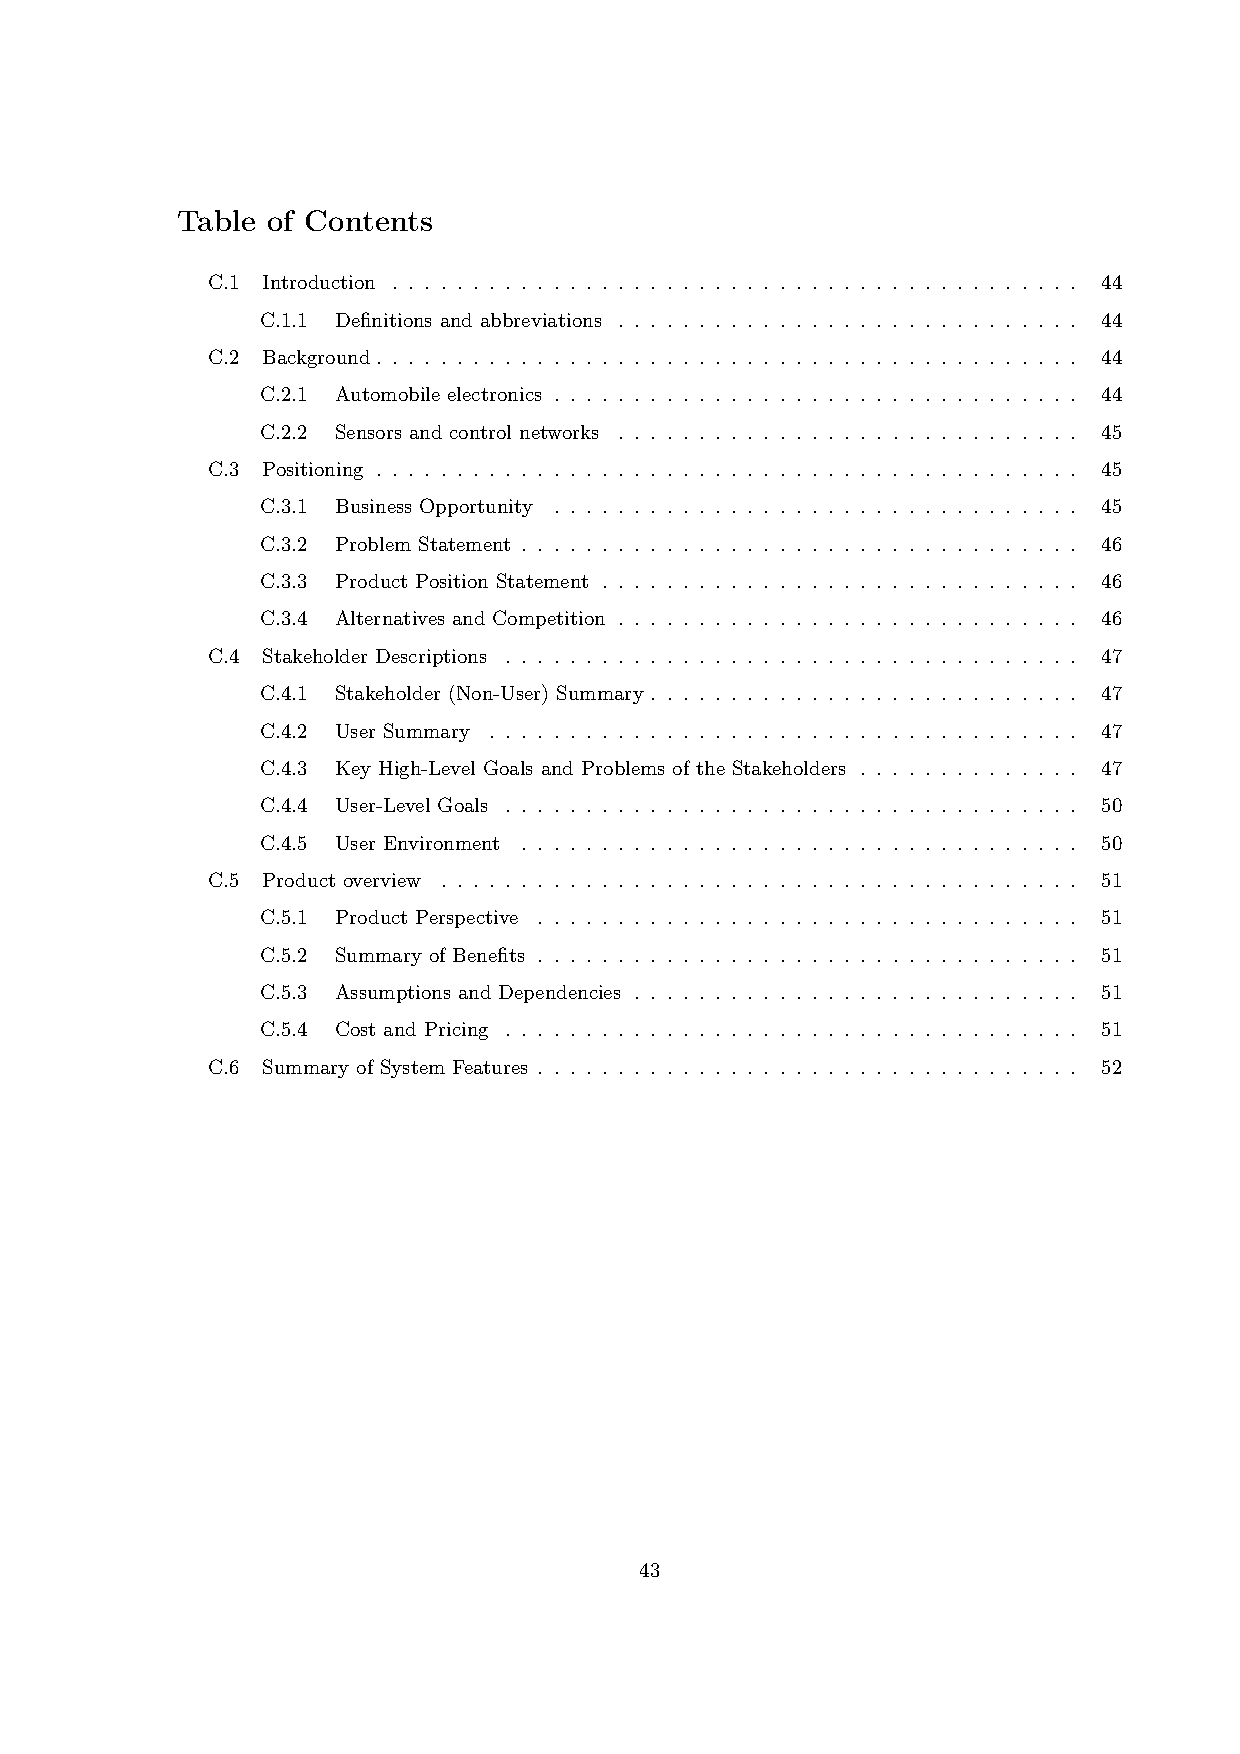
\includepdf[link,pages={-}]{output/vision.pdf}
%
%
%\chapter{System Requirements Document}
%\label{appendix:requirements}
%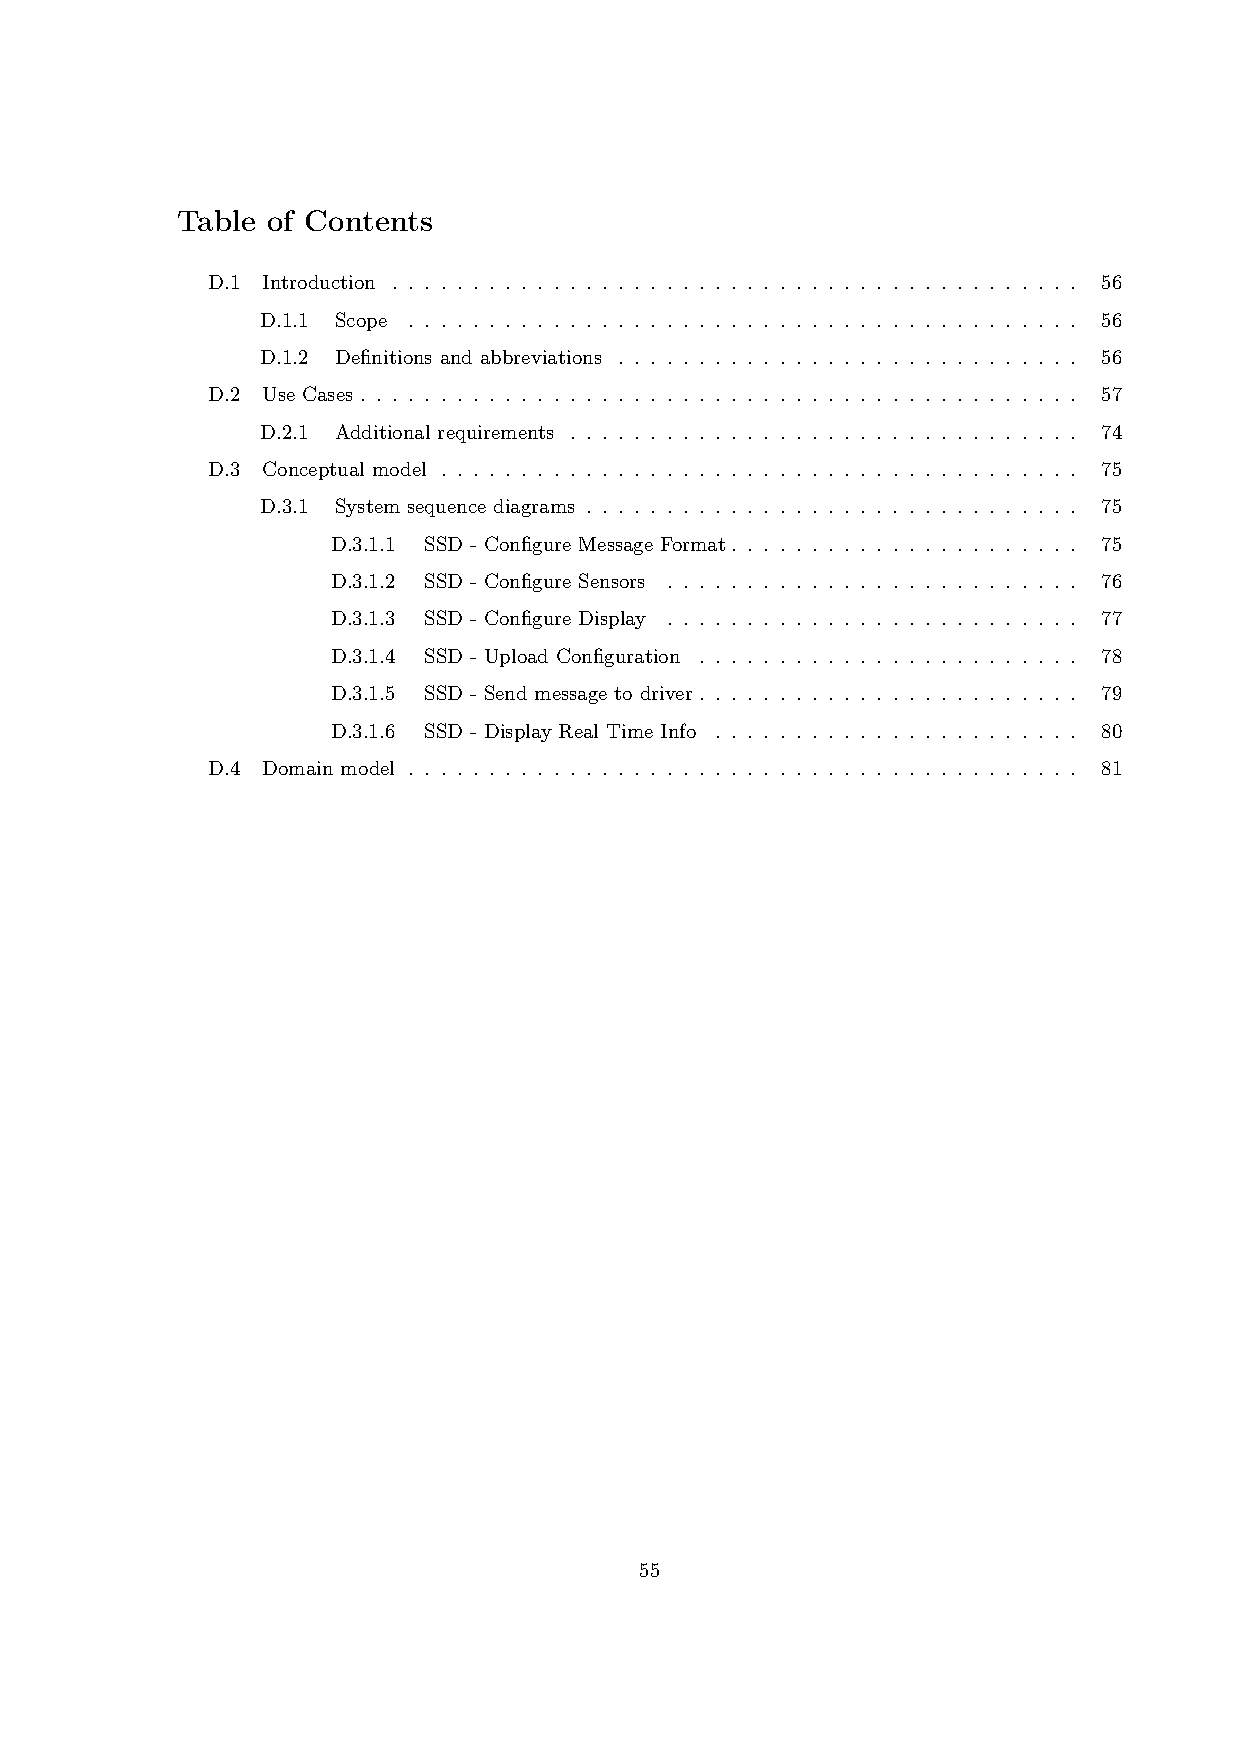
\includepdf[link,pages={-}]{output/requirements.pdf}
%
%
%\chapter{Supplementary Specification Document}
%\label{appendix:supspec}
%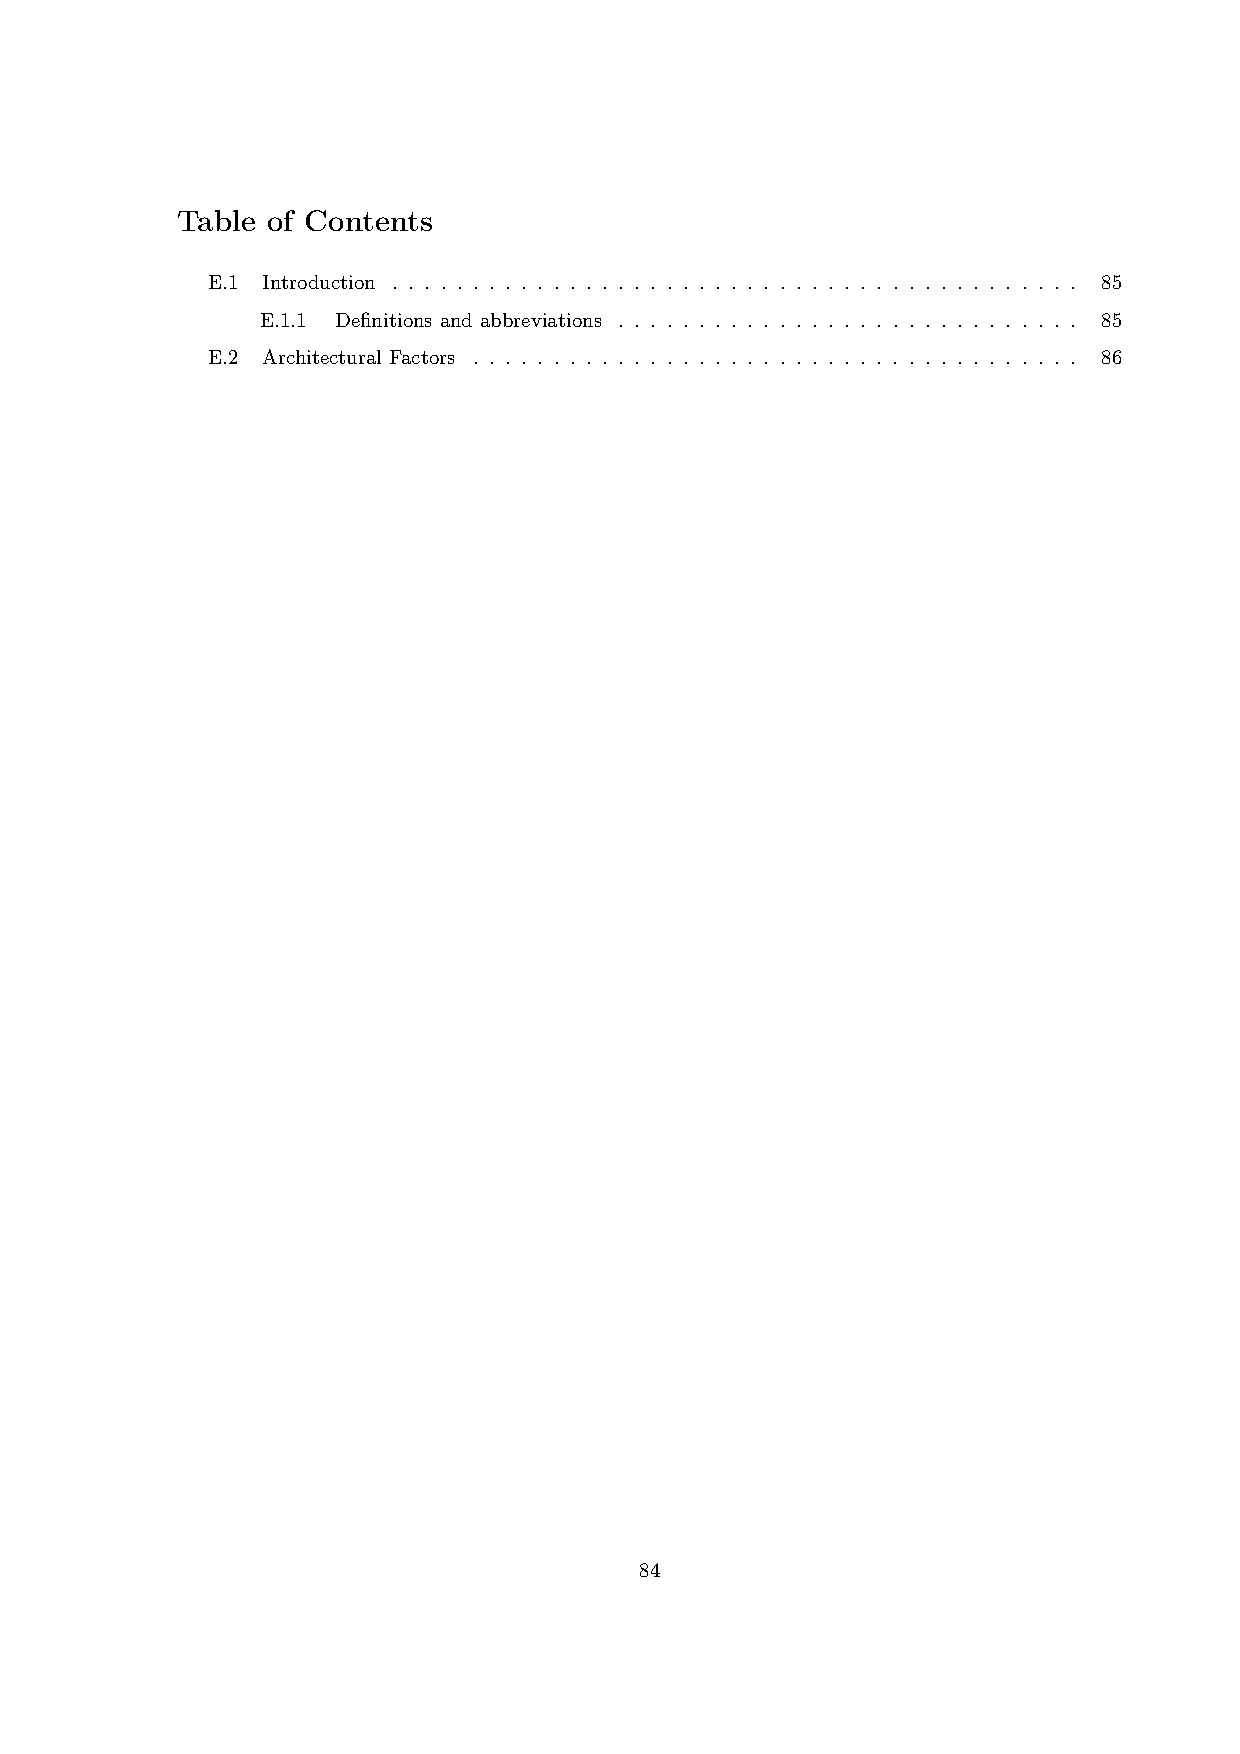
\includepdf[link,pages={-}]{output/supspec.pdf}
%
%\chapter{System Architecture Document}
%\label{appendix:sad}
%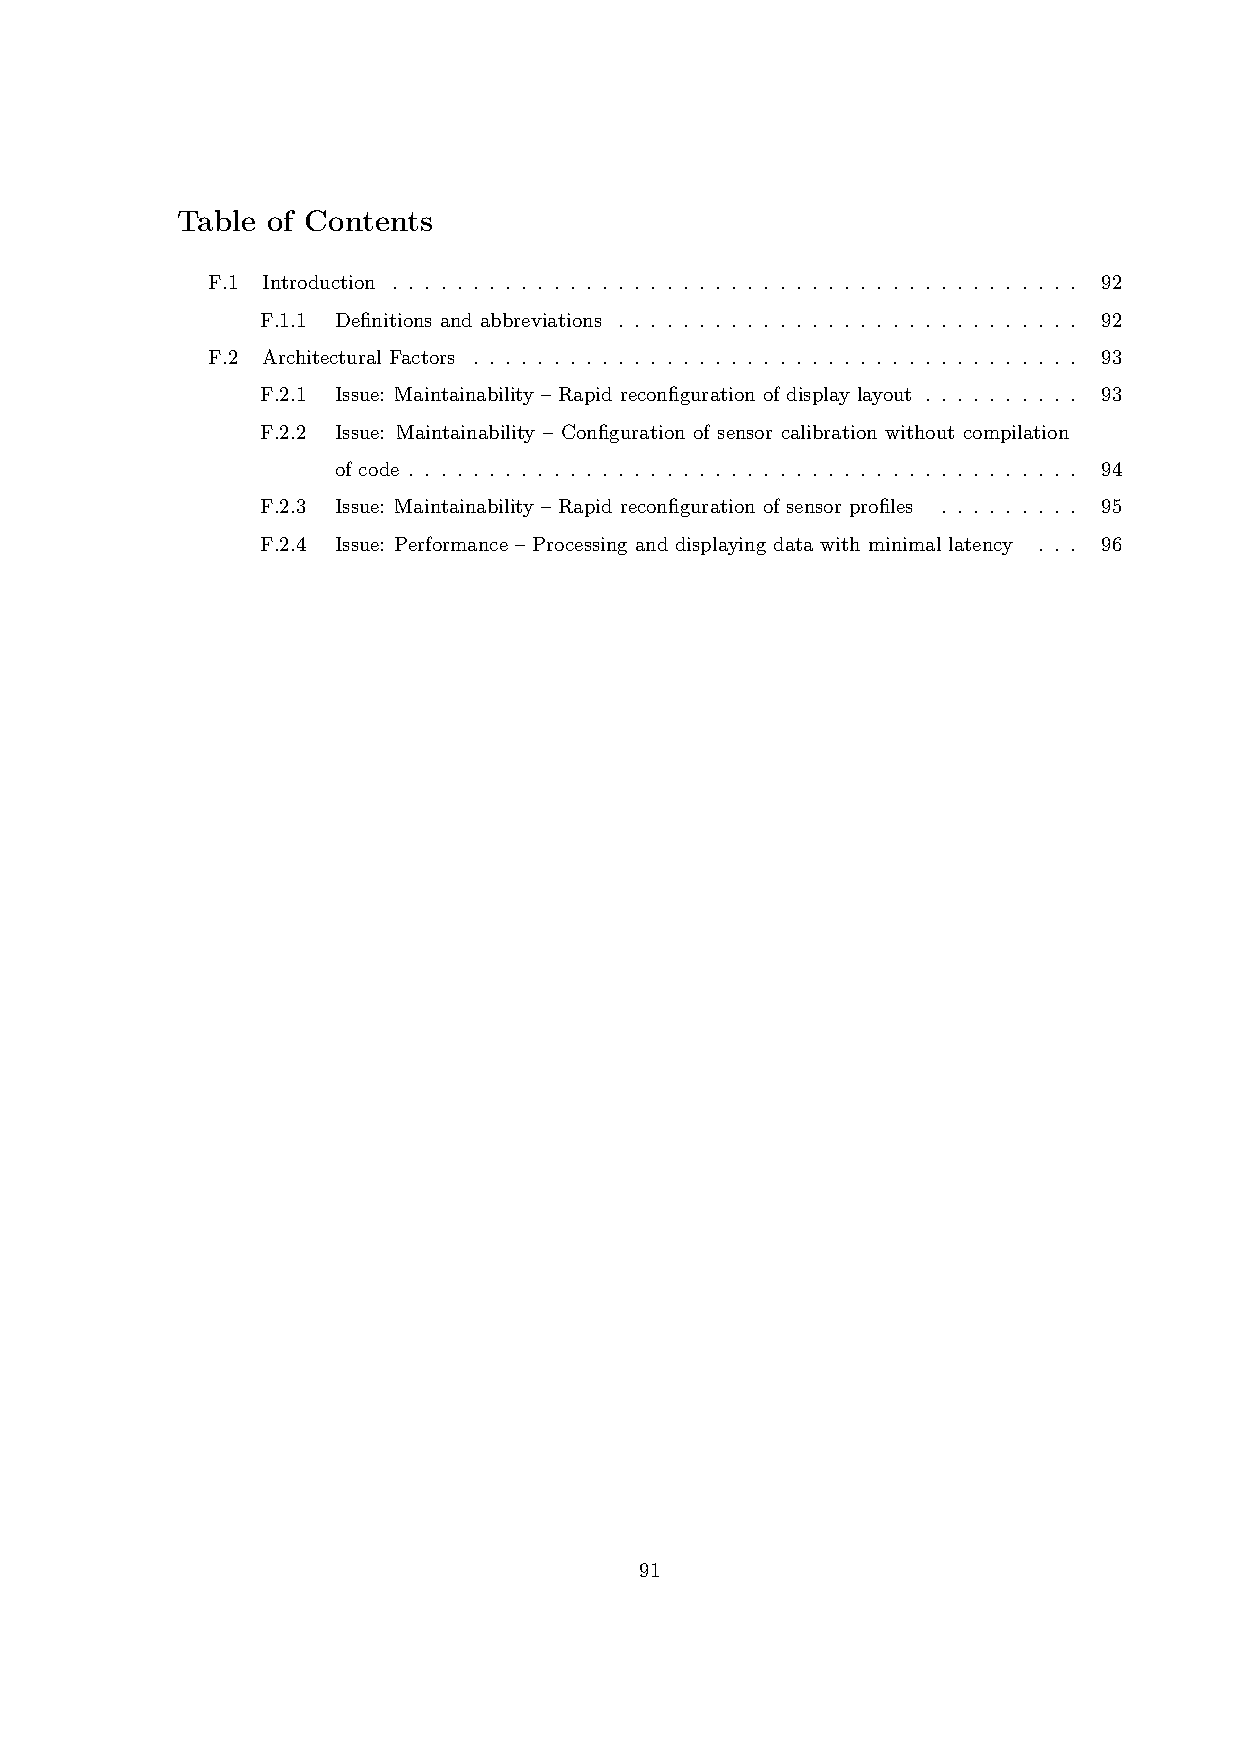
\includepdf[link,pages={-}]{output/architecture.pdf}

%\include{acronyms}
%\section{Attachments}
	\label{sec:attachments}

\subsection{U file for hydraulic piston case.}
\subsection{p file for hydraulic piston case.}
\subsection{pointMotionU file for hydraulic piston case.}
\subsection{blockMeshDict file for for hydraulic piston case.}

\subsection{U file for dynamic simulation of the concentric cylinder case.}
\subsection{p file for dynamic simulation of the concentric cylinder case.}
\subsection{pointDisplacement file for dynamic simulation of the concentric cylinder case.}
\subsection{blockMeshDict file for dynamic simulation of the concentric cylinder case.}
\subsection{controlDict file for dynamic simulation of the concentric cylinder case.}
\subsection{forces file for dynamic simulation of the concentric cylinder case.}

\subsection{angularOscillatingDisplacementPointPatchVectorField.C file.}
\subsection{oscillatingDisplacementPointPatchVectorField.C file.}
\subsection{libMyFunctionDisplacementPointPatchVectorField.C file.}

\subsection{Matlab script for generating .dat file for use in pointMotionU file.}
\subsection{pointDisplacement file for use with modified library.}
\subsection{Matlab script for plotting of analytical solution for pressure gradient.}
\subsection{Matlab script for autogeneration of simulated velocity profiles.}
\subsection{Matlab script for autogeneration of simulated force plots.}
%\includepdf[pages={-}]{} Legge til pdf


\end{document}
